\documentclass[12pt,oneside]{uhthesis}
\usepackage{subfigure}
\usepackage[ruled,lined,linesnumbered,titlenumbered,algochapter,spanish,onelanguage]{algorithm2e}
\usepackage{amsmath}
\usepackage{amssymb}
\usepackage{amsbsy}
\usepackage{caption,booktabs}
\captionsetup{ justification = centering }
%\usepackage{mathpazo}
\usepackage{float}
\setlength{\marginparwidth}{2cm}
\usepackage{todonotes}
\usepackage{listings}
\usepackage{xcolor}
\usepackage{multicol}
\usepackage{graphicx}

\usepackage{multirow} 
\usepackage{array}    
\usepackage{booktabs} 

\floatstyle{plaintop}
\restylefloat{table}
\addbibresource{Bibliography.bib}
% \setlength{\parskip}{\baselineskip}%
\renewcommand{\tablename}{Tabla}
\renewcommand{\listalgorithmcfname}{Índice de Algoritmos}
%\dontprintsemicolon
\SetAlgoNoEnd

\definecolor{codegreen}{rgb}{0,0.6,0}
\definecolor{codegray}{rgb}{0.5,0.5,0.5}
\definecolor{codepurple}{rgb}{0.58,0,0.82}
\definecolor{backcolour}{rgb}{0.95,0.95,0.92}

\lstdefinestyle{mystyle}{
    backgroundcolor=\color{backcolour},   
    commentstyle=\color{codegreen},
    keywordstyle=\color{purple},
    numberstyle=\tiny\color{codegray},
    stringstyle=\color{codepurple},
    basicstyle=\ttfamily\footnotesize,
    breakatwhitespace=false,         
    breaklines=true,                 
    captionpos=b,                    
    keepspaces=true,                 
    numbers=left,                    
    numbersep=5pt,                  
    showspaces=false,                
    showstringspaces=false,
    showtabs=false,                  
    tabsize=4
}

\lstset{style=mystyle}

\title{Mejoramiento del contraste de tomografía de cráneo con transformada synchrosqueezed}
\author{\\\vspace{0.25cm}Pedro Pablo Álvarez Portelles}
\advisor{\\\vspace{0.25cm}Dr.C. Damian Valdés Santiago}
\degree{Licenciado en Ciencia de la Computación}
\faculty{Facultad de Matemática y Computación}
\date{10 de junio de 2025\\\vspace{0.25cm}\href{https://github.com/ppalvar/thesis}{github.com/ppalvar/thesis}}
\logo{Graphics/uhlogo}
\makenomenclature

\renewcommand{\vec}[1]{\boldsymbol{#1}}
\newcommand{\diff}[1]{\ensuremath{\mathrm{d}#1}}
\newcommand{\me}[1]{\mathrm{e}^{#1}}
\newcommand{\pf}{\mathfrak{p}}
\newcommand{\qf}{\mathfrak{q}}
%\newcommand{\kf}{\mathfrak{k}}
\newcommand{\kt}{\mathtt{k}}
\newcommand{\mf}{\mathfrak{m}}
\newcommand{\hf}{\mathfrak{h}}
\newcommand{\fac}{\mathrm{fac}}
\newcommand{\maxx}[1]{\max\left\{ #1 \right\} }
\newcommand{\minn}[1]{\min\left\{ #1 \right\} }
\newcommand{\lldpcf}{1.25}
\newcommand{\nnorm}[1]{\left\lvert #1 \right\rvert }
\renewcommand{\lstlistingname}{Ejemplo de código}
\renewcommand{\lstlistlistingname}{Ejemplos de código}

\begin{document}

% \frontmatter
\maketitle

% \begin{dedication}
    Dedicado a mi madre, mi hermana, mi padre, mi familia y al amor de mi vida: los que han estado y estarán siempre conmigo.
\end{dedication}
% \begin{acknowledgements}
    Expreso mi agradecimiento a la Universidad de La Habana y a su claustro de profesores, quienes con dedicación y entrega me han guiado hacia metas que en un principio parecían inalcanzables. Agradezco también a mis compañeros y amigos por su apoyo constante a lo largo de esta etapa. De manera especial, deseo reconocer la orientación y el acompañamiento de mi tutor, cuyo consejo ha sido fundamental para la realización de este trabajo.
\end{acknowledgements}
% \begin{opinion}
    El uso de medios de contraste radiológicos en tomografía computarizada (TC) cerebral conlleva riesgos iatrogénicos significativos, como nefrotoxicidad, reacciones alérgicas e interferencias metabólicas, particularmente en pacientes con insuficiencia renal o comorbilidades. Estos efectos adversos justifican el empleo de métodos de mejoramiento digital del contraste o técnicas de inteligencia artificial, que permiten realzar estructuras anatómicas sin necesidad de aumentar la dosis de contraste.

    En particular, la transformada curvelet destaca en el procesamiento de imágenes de TC cerebral por su capacidad para representar eficientemente características morfológicas complejas. Su sensibilidad direccional multiescala permite capturar bordes curvilíneos y estructuras anatómicas finas, mejorando la detección de patologías. Además, su diseño anisotrópico separa eficazmente señal y ruido, preservando detalles clínicamente relevantes mientras reduce artefactos, optimizando tareas como segmentación, reconstrucción comprimida y mejora de contraste.

    Por su parte, la transformada synchrosqueezed (SST) ofrece alta resolución tiempo-frecuencia, descomponiendo señales no estacionarias con precisión. Localiza y separa componentes espectrales superpuestos, identificando patrones sutiles asociados a patologías. Su capacidad para reducir ruido manteniendo bordes y texturas la hace ideal para realzar estructuras cerebrales sin artefactos, siendo útil en diagnóstico asistido y procesamiento avanzado.

    El objetivo de la tesis fue desarrollar un método numérico basado en SST aplicada a curvelets (2DCT) para mejorar la calidad de imágenes de tomografía computarizada del cerebro, con especial énfasis en la visualización de tejidos blandos y lesiones pequeñas sin necesidad de agentes de contraste.

    La investigación realizada mostró que ventajas y desventajas del uso de este enfoque, que es una alternativa de menores prestaciones computacionales con respecto a las técnicas de inteligencia artificial, que no requiere un entrenamiento previo de modelos. Se recomienda continuar el trabajo en las áreas de mejora identificadas, tomando en cuenta el criterio cualitativo brindado por los especialistas.

    La tesis forma parte de las tareas de un proyecto nacional del CITMA para desarrollar algoritmos que aplican transformadas tiempo-frecuencia para analizar imágenes médicas, que incluye especialistas de alto nivel en diversas instituciones de salud cubanas y profesores e investigadores de nuestra facultad.

    Para esta tesis Pedro tuvo que estudiar las materias referidas, no incluidas en el currículo de la carrera, mostró disciplina, entrega y rigor. Además, demostró habilidades para el trabajo con la bibliografía y creatividad para proponer soluciones a problemas de implementación, entre otras competencias de programación en el lenguaje Python y sus diversos frameworks. En suma, considero que el estudiante logró cumplir el objetivo.

    \vspace{0.5cm}

    Por tanto, considero que a esta tesis del estudiante Pedro Pablo Álvarez Portelles debe otorgársele la máxima calificación (5 puntos, Excelente), y estoy seguro que en el futuro Pedro se desempeñará como un excelente profesional de la Computación.

    \vspace{1cm}

    \noindent
    Dr.C. Damian Valdés Santiago \\
    MSc. Dra. Lisbel Garzón Cutiño

    \vspace{0.5cm}

    \noindent
    13 de junio de 2025
\end{opinion}
% \begin{resumen}
	La tomografía computarizada de cráneo es una herramienta esencial en el diagnóstico de patologías intracraneales, aunque su utilidad puede verse limitada por la presencia de imágenes con bajo contraste, especialmente en regiones de tejidos blandos y estructuras anatómicas sutiles. En este trabajo se propone el uso de la transformada \textit{synchrosqueezed}, una técnica avanzada de procesamiento de señales, para mejorar la representación tiempo-frecuencia de la descomposición resultante de una transformada \textit{curvelet} 2D. A diferencia de métodos tradicionales de mejora de imagen, SST permite una descomposición más precisa de componentes morfológicos y una reconstrucción adaptativa, lo que preserva bordes y texturas críticas para el diagnóstico.  El estudio incluyó un análisis estadístico, donde se calcularon métricas cuantitativas. Adicionalmente, se realizó una validación cualitativa por parte de una especialista.

	El método propuesto constituye una alternativa efectiva y accesible para el mejoramiento del contraste en imágenes de tomografía computarizada de cráneo, especialmente útil en situaciones donde no es posible el uso de agentes de contraste o tecnologías de inteligencia artificial avanzadas. Los resultados obtenidos evidencian que es posible realzar detalles anatómicos clínicamente relevantes, como lesiones pequeñas y estructuras de bajo contraste, sin introducir artefactos visuales significativos ni comprometer la integridad de la imagen original.
\end{resumen}

\begin{abstract}
	Cranial computed tomography is an essential tool in the diagnosis of intracranial pathologies, although its usefulness may be limited by the presence of low-contrast images, especially in soft tissue regions and subtle anatomical structures. This work proposes the use of the \textit{synchrosqueezed} transform, an advanced signal processing technique, to improve the time-frequency representation of the decomposition resulting from a 2D \textit{curvelet} transform. Unlike traditional image enhancement methods, SST allows for a more precise decomposition of morphological components and adaptive reconstruction, preserving edges and textures critical for diagnosis. The study included a statistical analysis, where quantitative metrics were calculated. Additionally, qualitative validation was performed by a specialist.

	The proposed method constitutes an effective and accessible alternative for contrast enhancement in cranial computed tomography images, particularly useful in situations where the use of contrast agents or advanced artificial intelligence technologies is not feasible. The obtained results demonstrate that it is possible to enhance clinically relevant anatomical details, such as small lesions and low-contrast structures, without introducing significant visual artifacts or compromising the integrity of the original image.
\end{abstract}
% \include{FrontMatter/Contents}

\mainmatter

\chapter{Detalles de Implementación y Experimentos}\label{chapter:implementation}

En este capítulo se describe detalladamente el proceso de implementación del método propuesto para la mejora de imágenes de tomografía computarizada cerebral. Se presentan las herramientas y entornos de desarrollo empleados, así como las adaptaciones realizadas sobre las implementaciones existentes de la transformada synchrosqueezed (SST) y su inversa (ISST) en el contexto de la transformada curvelet bidimensional (2DCT). Además, se explican los procedimientos seguidos para el preprocesamiento de los datos, la configuración de los experimentos y la aplicación de las distintas estrategias de modificación de la matriz de energía. Finalmente, se justifica la selección de los parámetros experimentales y se expone la estructura general del flujo de trabajo, sentando las bases para la posterior evaluación y comparación de los resultados obtenidos.

\section{Ambiente de trabajo y herramientas}\label{section:work-environment}

El funcionamiento principal de los experimentos gira alrededor de la implementación original de las funciones de SST e ISST, por Haizhao Yang y Lexing Ying \cite{SynchrosqueezedCurveletTransform_SynLab}. Esta fue originalmente concebida en \texttt{Matlab}, un software y lenguaje de programación matemático, con gran énfasis en la practicidad y en la facilidad de uso para personal del sector científico. Esta implementación, con cambios mínimos, fue exportada a \texttt{GNU Octave}, una versión gratuita y de código abierto creada y mantenida por una extensa comunidad de contribuidores. Esto se hizo con el objetivo de poder utilizarlo sin la restricción de las barreras de pago, que en nuestro país se hace de gran dificultad. Esta implementación se encuentra modularizada en el repositorio de la tesis.

Dada la elevada dificultad de la implementación de SST y de ISST, además de la complejidad para crear experimentos complejos y paralelizables para mejor rendimiento, esta fue usada solo como una librería dinámica la cual fue llamada desde \texttt{Python 3.13}. Para esto, se usó la librería \texttt{oct2py}, la cual permite integración directa con el motor de \texttt{Octave} para llamar a las funciones definidas (en este caso solo SST e ISST) con objetos nativos de \texttt{Python}, como son arreglos n-dimensionales de \texttt{numpy}.

Durante el desarrollo y la ejecución de los experimentos, el código fue implementado y ejecutado íntegramente en la unidad central de procesamiento (CPU) de un equipo portátil de alto rendimiento. Este sistema cuenta con un procesador AMD Ryzen 7 8845HS de 8 núcleos y 16 hilos, con una frecuencia base de 3.8 GHz y una frecuencia máxima de hasta 5.1 GHz. Además, dispone de 32 GB de memoria RAM DDR5 y una unidad de almacenamiento sólido (SSD) de 1 TB. Todas las tareas de procesamiento, incluidas las etapas más intensivas computacionalmente, se realizaron exclusivamente en la CPU, sin recurrir a aceleración por hardware gráfico. Estas especificaciones proporcionaron un entorno adecuado para evaluar el rendimiento y la escalabilidad de la implementación propuesta, asegurando resultados reproducibles y tiempos de ejecución competitivos.

Adicionalmente, para el manejo, procesamiento y análisis de los resultados, se emplearon diversas herramientas del ecosistema científico de Python, tales como \texttt{numpy} para operaciones matriciales y de álgebra lineal, \texttt{matplotlib} para la visualización de datos y \texttt{pandas} para la manipulación de conjuntos de datos. El desarrollo de scripts experimentales, automatización de pruebas y gestión de resultados se realizó en un entorno de desarrollo basado en \texttt{Jupyter Notebook}, lo que facilitó la documentación interactiva y la reproducibilidad de los experimentos. Para el control de versiones y la colaboración, se utilizó el sistema \texttt{git}, permitiendo un seguimiento detallado de los cambios y la integración eficiente de mejoras en el código fuente. Finalmente, la ejecución de los experimentos se gestionó mediante scripts de automatización en \texttt{bash} y el uso de entornos virtuales con \texttt{conda} para asegurar la compatibilidad y portabilidad de las dependencias empleadas a lo largo del proyecto.

Para garantizar la reproducibilidad de los resultados y la consistencia en los experimentos, se fijaron explícitamente las semillas aleatorias y las configuraciones relevantes en todos los procesos. Esto permitió obtener resultados comparables y facilitar la validación de los procedimientos implementados.

\section{Optimización de la implementación}\label{section:optimization}

Con el objetivo de mejorar la eficiencia y el rendimiento de la solución propuesta, se han incorporado las siguientes optimizaciones en la implementación:

\begin{itemize}
    \item \textbf{Caché de los datos obtenidos:} Se ha implementado un sistema de almacenamiento temporal de los datos intermedios, como son el resultado de aplicar SST sobre una imagen en particular. Esta estrategia permite reutilizar resultados previamente calculados y reducir el acceso a la memoria principal o la necesidad de recomputar información, lo que se traduce en una disminución significativa del tiempo de ejecución global.
    
    \item \textbf{Paralelización de la ejecución:} Se ha aprovechado la capacidad de procesamiento concurrente de \texttt{Python} mediante la paralelización del procesamiento de imágenes independientes. Esto permite distribuir la carga de trabajo entre múltiples núcleos o hilos, acelerando etapas críticas como el cálculo de transformadas y la reconstrucción de imágenes, y logrando una mejora sustancial en los tiempos de cómputo.
    
    \item \textbf{Limpieza de los objetos no utilizados en memoria:} Para evitar la acumulación innecesaria de datos y prevenir posibles fugas de memoria, se ha incorporado un mecanismo de liberación sistemática de los objetos que ya no son requeridos durante la ejecución. Esta gestión eficiente de la memoria contribuye a mantener la estabilidad y el rendimiento de la aplicación, especialmente en experimentos de gran escala o en entornos con recursos limitados.
\end{itemize}

La necesidad de implementar optimizaciones en el procesamiento de imágenes surge de las exigencias computacionales observadas durante el desarrollo experimental. En primer lugar, el resultado de la SST aplicada a una sola imagen puede ocupar aproximadamente 1.4 GB de espacio en memoria, lo que representa una carga significativa para los recursos del sistema. Además, los tiempos de ejecución para el procesamiento completo de una imagen —incluyendo tanto la SST como su inversa (ISST)— alcanzan una media de 4 minutos, lo que limita la viabilidad del método en escenarios donde se requiere el análisis de grandes volúmenes de datos o la respuesta en tiempo real. Por otro lado, el consumo de memoria RAM sin la aplicación de optimizaciones puede llegar a ser muy intenso, alcanzando picos de hasta 15 GB durante la ejecución de múltiples experimentos. Estas condiciones motivan la incorporación de técnicas específicas de optimización, orientadas a reducir el uso de memoria, agilizar los tiempos de procesamiento y garantizar la estabilidad del sistema, permitiendo así la aplicación práctica y eficiente del método propuesto en entornos computacionales con recursos limitados.

Como resultado de las optimizaciones implementadas, se logró una reducción significativa tanto en los tiempos de ejecución como en el consumo de memoria del sistema. Tras la aplicación de estas mejoras, el tiempo medio de procesamiento por experimento —incluyendo la aplicación de SST e ISST sobre una imagen— disminuyó a aproximadamente 2 minutos, lo que representa una mejora sustancial en la eficiencia operativa del método. Asimismo, el uso máximo de memoria RAM durante la ejecución se redujo a 4 GB, permitiendo la realización de experimentos en equipos con recursos más limitados y mejorando la estabilidad general del sistema durante la ejecución de múltiples tareas en paralelo. Estos resultados evidencian la efectividad de las estrategias de optimización adoptadas en el desarrollo de la presente implementación.

\section{Implementación de los experimentos} \label{section:experiment-implementation}

La implementación de los experimentos se basa en un flujo modular que permite el procesamiento eficiente y reproducible de imágenes. El proceso inicia con la carga y normalización de las imágenes, que pueden provenir tanto de archivos individuales en formatos estándar (\texttt{.jpg} o \texttt{png}) como de volúmenes médicos (\texttt{.nii}). Para la gestión y muestreo de imágenes, se emplean objetos utilitarios que permiten recuperar conjuntos de imágenes desde directorios estructurados, facilitando la selección aleatoria o secuencial de muestras para los experimentos.

En cuanto al preprocesamiento, este se aplicó de manera diferenciada según la naturaleza de los experimentos. En una primera serie de experimentos, las imágenes fueron normalizadas para que sus valores de intensidad se encontraran en el rango $[0, 1]$. Esta normalización permitió asegurar la homogeneidad en la escala de entrada y facilitó la comparación directa entre diferentes muestras, independientemente de su origen o condiciones de adquisición.

En una segunda serie de experimentos, se utilizaron imágenes volumétricas en formato \texttt{.nii}, sobre las cuales se aplicó una ventana de intensidad específica para procesar únicamente la sección correspondiente a la densidad del cerebro. Esta técnica de ventana permitió resaltar las estructuras anatómicas de interés y reducir el impacto de regiones irrelevantes o valores atípicos, optimizando así la calidad y relevancia de los datos utilizados en el análisis posterior.

Cabe destacar que la naturaleza del preprocesamiento aplicado influyó notablemente en los tiempos de ejecución de los experimentos. En la primera serie, al trabajar con imágenes normalizadas en un rango reducido de valores, los tiempos de procesamiento fueron considerablemente menores, con una media aproximada de 1 minuto por experimento. En contraste, la segunda serie, basada en imágenes volumétricas procesadas mediante la aplicación de una ventana de intensidad, presentó tiempos de ejecución significativamente mayores, oscilando entre 3 y 5 minutos por experimento. Esta diferencia en el rendimiento también tuvo implicaciones directas en los resultados obtenidos, las cuales serán analizadas en detalle en una sección posterior.% todo

Una vez cargadas y preprocesadas, las imágenes son transformadas mediante la aplicación de la transformada synchrosqueezed curvelet y su inversa. Este procedimiento se encuentra encapsulado en objetos que gestionan tanto la ejecución de las transformadas como la utilización de un sistema de caché, el cual almacena los resultados intermedios para evitar recomputaciones innecesarias y optimizar el uso de recursos. Los resultados de la transformada se almacenan en estructuras especializadas que contienen la energía synchrosqueezed, los coeficientes curvelet y los vectores asociados, permitiendo su manipulación eficiente en las siguientes etapas del experimento.

Las funciones experimentales, están implementadas como procedimientos puros que operan sobre los resultados de la transformada, generando nuevas instancias modificadas de dichos resultados sin alterar los datos originales. La ejecución de cada experimento se gestiona a través de utilidades que reciben una configuración detallada, especificando la función experimental a aplicar, los parámetros y los argumentos adicionales requeridos. Tras la aplicación de la función experimental, se realiza la reconstrucción de la imagen modificada mediante la transformada inversa, asegurando la consistencia del flujo de procesamiento.

Durante todo el proceso, se implementa un sistema de registro para el seguimiento detallado de cada etapa y la gestión de errores. Además, se asegura la reproducibilidad de los experimentos mediante la fijación de semillas aleatorias y la serialización de los resultados y configuraciones empleadas. Este enfoque modular y estructurado permite realizar experimentos complejos de manera eficiente, garantizando la trazabilidad y la robustez de los resultados obtenidos.

El flujo completo de procesamiento experimental se organiza a través de una función principal que recibe como entrada un conjunto de imágenes, las configuraciones específicas de los experimentos a realizar y las configuraciones de las métricas de evaluación. Internamente, esta función itera sobre cada imagen y, para cada una, aplica de manera secuencial las distintas configuraciones experimentales definidas. Para cada combinación de imagen y configuración experimental, se ejecuta el procesamiento correspondiente: primero se realiza la transformada synchrosqueezed sobre la imagen, luego se aplica la función experimental seleccionada sobre los resultados de la transformada, y finalmente se reconstruye la imagen modificada mediante la transformada inversa.

Durante este proceso, se calculan las métricas de evaluación especificadas, comparando la imagen reconstruida con la original u otras referencias según corresponda. Todos los resultados, así como los parámetros y configuraciones utilizados, se almacenan y registran de forma estructurada para su posterior análisis. Este proceso automatizado permite ejecutar grandes volúmenes de experimentos de manera eficiente, garantizando la trazabilidad y la reproducibilidad (ver imagen \ref{fig:diagrama-flujo-experimentos}).

\begin{figure}[H]
    \centering
    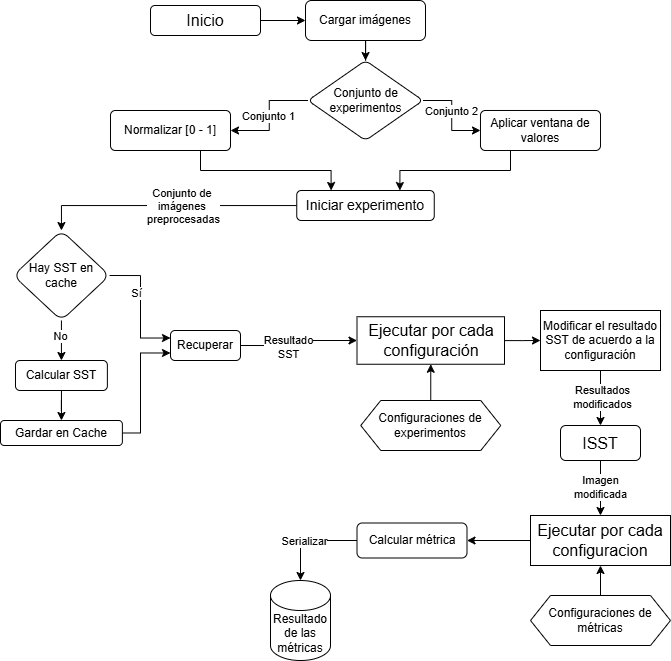
\includegraphics[width=0.95\textwidth]{Graphics/diagrama experimentos tesis.drawio.png}
    \caption{Diagrama de flujo del pipeline experimental implementado para el procesamiento y análisis de imágenes.}
    \label{fig:diagrama-flujo-experimentos}
\end{figure}

\begin{table}[h]
    \centering
    \caption{Configuraciones experimentales y sus parámetros.\cite{ExperimentSource,ExperimentSource2}}
    \label{tab:experimentos}
    \begin{tabular}{>{\raggedright}p{4cm}p{6cm}}
    \toprule
    \textbf{Tipo de Experimento} & \textbf{Parámetros} \\ 
    \midrule
    Umbralizado & threshold = 0.1, 0.05, 0.001 \\
    \midrule
    Mejora de energía & \texttt{enhancement\_factor} = 3.0, 1.5, 10 \\
    \midrule
    Filtro pasa-alto & \texttt{cutoff\_scale} = 5, 10 \\
    \midrule
    Filtro pasa-banda & \texttt{low\_scale} = 5 (\texttt{high\_scale} = 10), 15 (20) \\
    \midrule
    Máscara gaussiana & $ \mu  = N/2$, $ \sigma $ = 1.0, 4.0, 6.0 \\
    \midrule
    Máscara exponencial & \texttt{decay\_rate} = 0.1, 0.01 \\
    \bottomrule
    \end{tabular}
    \footnotesize{\\*N/2: mitad de las escalas disponibles en la descomposición.}
\end{table}

Para la realización de los experimentos se utilizó un conjunto de configuraciones específicas, las cuales se detallan en la Tabla~\ref{tab:experimentos}. Cada configuración define los parámetros y valores empleados en las distintas funciones experimentales aplicadas durante el procesamiento, permitiendo así evaluar el comportamiento del método bajo diferentes condiciones y ajustes. Esta variedad de configuraciones facilita un análisis exhaustivo y comparativo de los resultados obtenidos.

\section{Implementación de las métricas} \label{section:metrics-implementation}

Las métricas utilizadas para la evaluación cuantitativa de los resultados experimentales fueron implementadas de manera modular y eficiente, empleando herramientas especializadas del ecosistema científico de \texttt{Python}. Las configuraciones específicas de las métricas se encuentran detalladas en la Tabla~\ref{tab:metricas}

Para las métricas basadas en operaciones numéricas y estadísticas, como el índice de mejora de contraste y la razón de nitidez basada en el operador Laplaciano, se utilizó la biblioteca \texttt{numpy} para el cálculo vectorizado de desviaciones estándar y varianzas, así como \texttt{opencv-python} para la aplicación de operadores de filtrado espacial.

Las métricas perceptuales avanzadas, como el FSIM (Feature Similarity Index) y LPIPS (Learned Perceptual Image Patch Similarity), se implementaron a través de las bibliotecas \texttt{piq} y \texttt{lpips}, respectivamente, haciendo uso de \texttt{PyTorch} para el manejo de tensores y la ejecución eficiente en CPU. El índice de similitud estructural (SSIM) y la relación señal-ruido pico (PSNR) se calcularon utilizando las funciones \texttt{structural\_similarity} y \texttt{peak\_signal\_noise\_ratio} de la biblioteca \texttt{scikit-image}. Para la métrica BRISQUE, orientada a la evaluación de artefactos y ruido perceptual, se empleó la implementación disponible en \texttt{piq}.

El flujo de cálculo de métricas se integra al final de cada experimento: una vez reconstruida la imagen modificada, se aplican de forma automática todas las métricas relevantes, comparando la imagen procesada con la original o con una referencia apropiada (en este caso, con la imagen original). Cada función de métrica está desacoplada del resto del procesamiento y recibe como entrada los arreglos de imagen en formato \texttt{numpy}, asegurando así su reutilización y extensibilidad.

Los resultados de cada métrica, junto con la configuración experimental correspondiente, son almacenados y registrados de forma estructurada al finalizar cada experimento. Este enfoque garantiza la trazabilidad y facilita el análisis comparativo entre diferentes configuraciones y tipos de preprocesamiento. Además, la modularidad de la implementación permite la fácil incorporación de nuevas métricas en futuras extensiones del trabajo.

De manera concreta, para cada imagen procesada, una vez ejecutados todos los experimentos definidos, se calculan de forma automática todas las métricas seleccionadas para cada resultado. Posteriormente, los valores obtenidos de las métricas, junto con la información sobre la imagen y la configuración experimental utilizada, son serializados y almacenados en un archivo en formato \texttt{json}. Esta estrategia permite centralizar y organizar los datos de evaluación, facilitando su análisis posterior, la comparación sistemática entre diferentes métodos y la integración con herramientas externas de análisis estadístico o visualización.

\begin{table}[h]
    \centering
    \caption{Métricas de evaluación agrupadas por categorías\cite{Metrics}}
    \label{tab:metricas}
    \begin{tabular}{p{3cm}p{8cm}p{3cm}}
    \toprule
    \textbf{Categoría} & \textbf{Métrica} & \textbf{Descripción} \\ 
    \midrule
    \multirow{3}{*}{Mejora} 
    & CII (\textit{Contrast Improvement Index}) & Índice de mejora de contraste \\
    & LSR (\textit{Laplacian Sharpness Ratio}) & Cociente de nitidez Laplaciana \\
    & FSIM (\textit{Feature Similarity Index}) & Similaridad de características \\
    \midrule

    \multirow{3}{*}{Distorsión}
    & PSNR (\textit{Peak Signal-to-Noise Ratio}) & Relación señal-ruido \\
    & SSIM (\textit{Structural Similarity Index}) & Similaridad estructural \\
    & LPIPS (\textit{Learned Perceptual Image Patch Similarity}) & Similaridad perceptual \\
    \midrule

    \multirow{2}{*}{Artefactos}
    & RNS (Residual Noise Standard Deviation) & Desviación estándar del ruido residual \\
    & BRISQUE (Blind/Referenceless Image Spatial Quality Evaluator \cite{BRISQUE}) & Evaluador ciego de calidad \\
    \bottomrule
    \end{tabular}
\end{table}

\section{Implementación de las estadísticas}\label{section:statistics-implementation}

El análisis estadístico de los resultados experimentales se diseñó para comparar de manera rigurosa el desempeño de los distintos métodos evaluados. Para cada par de experimentos a comparar, se recopilaron los valores obtenidos de las métricas correspondientes en todas las imágenes procesadas. El primer paso consistió en la aplicación de pruebas de normalidad sobre la distribución de cada métrica, con el objetivo de determinar el tipo de análisis estadístico adecuado para la comparación. Las pruebas de normalidad empleadas incluyeron, entre otras, la prueba de Shapiro-Wilk.

En función de los resultados de la prueba de normalidad, se seleccionó el método estadístico más apropiado para la comparación de los dos grupos experimentales. Cuando la distribución de las métricas fue compatible con la normalidad, se utilizó la prueba t de Student para muestras independientes, permitiendo evaluar si existían diferencias estadísticamente significativas entre las medias de los grupos. En caso contrario, es decir, si la distribución no era normal, se recurrió a pruebas no paramétricas como la prueba de Mann-Whitney U, que permite comparar la mediana de dos muestras independientes sin asumir normalidad.

Si el análisis estadístico indicó que existían diferencias significativas entre los experimentos comparados, se procedió a comparar sus medias y desviaciones estándar para cada métrica, determinando así cuál de los dos experimentos presentaba un mejor desempeño según los valores observados. En caso de que no se detectaran diferencias estadísticamente significativas, se asumió que ambos experimentos ofrecían resultados equivalentes para la métrica analizada.

\begin{table}[h]
    \centering
    \caption{Resumen de las métricas utilizadas, sus valores ideales y rangos de referencia.}
    \label{tab:metrics-expected-values}
    \begin{tabular}{>{\raggedright}p{5cm}p{3cm}p{3cm}}
        \toprule
        \textbf{Métrica} & \textbf{Valor ideal} & \textbf{Rango} \\
        \midrule
        Índice de mejora de contraste (CII) & $>1$ & $[0, \infty)$ \\
        Razón laplaciana & $>1$ & $[0, \infty)$ \\
        FSIM & $1$ & $[0, 1]$ \\
        PSNR & $\infty$ & $[0, \infty)$ \\
        SSIM & $1$ & $[0, 1]$ \\
        LPIPS & $0$ & $[0, 1]$ \\
        Desviación estándar del ruido residual & $0$ & $[0, \infty)$ \\
        BRISQUE & $0$ & $[0, 100]$ \\
        \bottomrule
    \end{tabular}
\end{table}

Adicionalmente, para cada métrica se consultó una tabla de valores esperados o ideales (Tabla~\ref{tab:metrics-expected-values}), lo que permitió contextualizar los resultados obtenidos y seleccionar el experimento más favorable dentro de cada par comparado. En este proceso, se otorgó un peso mayor a aquellas métricas consideradas prioritarias para la calidad de la imagen, como el índice de similitud estructural (SSIM), que evalúa la preservación de la estructura, y la métrica de nitidez basada en el operador Laplaciano, que prioriza la definición de bordes. Esta ponderación permitió orientar la selección final hacia los experimentos que maximizan la fidelidad estructural y la nitidez en las imágenes reconstruidas.

Para el análisis estadístico de los resultados experimentales se emplearon principalmente las bibliotecas \texttt{pandas} para la manipulación y análisis de los datos tabulados, y \texttt{scipy.stats} para la ejecución de pruebas estadísticas como el test de normalidad y las pruebas de comparación entre grupos. Adicionalmente, las bibliotecas \texttt{seaborn} y \texttt{matplotlib.pyplot} se utilizaron para la visualización gráfica de los resultados y la exploración de tendencias y distribuciones. Estas herramientas permitieron realizar un análisis estadístico riguroso, reproducible y visualmente comprensible de los datos obtenidos en los experimentos.

% \chapter{Marco teórico}\label{chapter:state-of-the-art}

En este capítulo se presentan los fundamentos teóricos necesarios para el desarrollo de esta investigación. Se abordan los principios del procesamiento digital de imágenes, con especial énfasis en las características y particularidades de las imágenes obtenidas por tomografía computarizada (TC) de cráneo. Asimismo, se describen las técnicas convencionales y actuales de mejora de contraste en imágenes médicas, destacando sus ventajas y limitaciones. Finalmente, se introduce el marco conceptual de la transformada synchrosqueezed, que servirá de base para la propuesta metodológica de mejoramiento de contraste desarrollada en este trabajo.

\section{Imágenes de CT}

En el contexto de esta tesis, una imagen digital se representa formalmente como una matriz $ M \in \mathbb{R}^{n \times m} $, donde cada elemento $ (i, j) $ corresponde a la intensidad o luminancia del píxel ubicado en la fila $ i $ y columna $ j $, $ n $ y $ m $ son las dimensiones de la imagen. En imágenes a color, la representación suele involucrar tres matrices independientes, cada una asociada a la intensidad de los canales rojo, verde y azul (RGB, por sus siglas en inglés). Sin embargo, dado que las imágenes de CT son inherentemente monocromáticas, una sola matriz es suficiente para describir la distribución de intensidades, lo que simplifica su procesamiento y análisis.%todo: poner ref 

En el caso particular de las imágenes médicas obtenidas mediante CT de cráneo \cite{Flandrin2018}, cada valor de la matriz representa la atenuación de los rayos X en una región específica del tejido, cuantificada mediante unidades Hounsfield (HU, por sus siglas en inglés). Estas unidades permiten distinguir entre diferentes tipos de tejidos, como hueso, sustancia gris, sustancia blanca y líquido cefalorraquídeo, en función de sus propiedades de absorción.%todo: poner ref

Durante la adquisición de imágenes de CT, se utiliza un equipo especializado compuesto por un escáner de gran tamaño con forma de anillo, denominado \textit{gantry}. El paciente se recuesta sobre una mesa motorizada que se desplaza lentamente a través del gantry, mientras un tubo de rayos X y un conjunto de detectores electrónicos rotan alrededor de la cabeza del paciente. Este sistema emite haces de rayos X que atraviesan los tejidos y son atenuados en función de sus propiedades físicas; los detectores captan la radiación remanente y envían la información a una computadora central.%todo: poner ref

\begin{figure}[H]
    \centering
    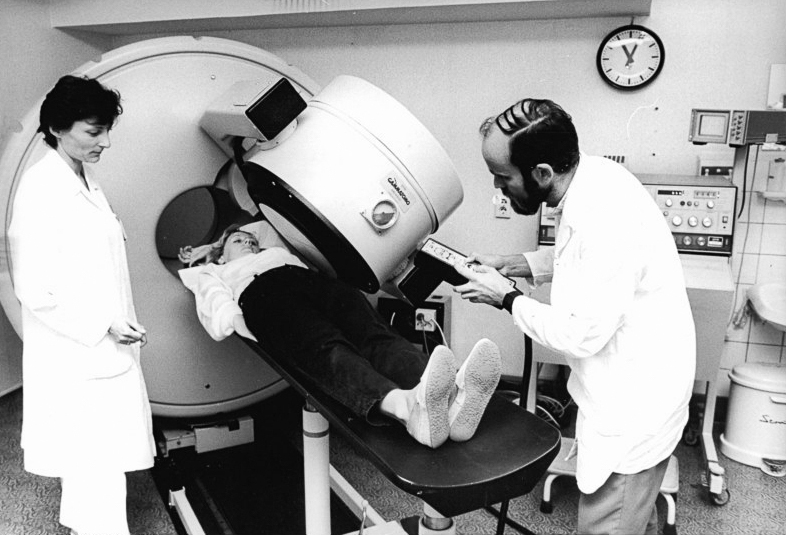
\includegraphics[width=0.95\textwidth]{Graphics/Bundesarchiv_Bild_183-1989-0921-014,_Schwerin,_Bezirkskrankenhaus,_Computertomograf.jpg}
    \caption{Paciente sometido a un examen de CT \cite{bundesarchiv1989}.}
    \label{fig:patient-ct-scan}
\end{figure}

La computadora procesa los datos recolectados durante las múltiples rotaciones y posiciones del tubo de rayos X, aplicando algoritmos matemáticos avanzados para reconstruir imágenes transversales o cortes bidimensionales del cráneo. Estas imágenes pueden ser posteriormente apiladas para obtener representaciones tridimensionales detalladas, lo que facilita la identificación precisa de estructuras anatómicas y posibles patologías.%todo: poner ref

En el desarrollo de esta tesis, las imágenes médicas utilizadas se almacenan y procesan en el formato NIfTI (\textit{Neuroimaging Informatics Technology Initiative} \cite{cox2004nifti}, con extensión de archivo \texttt{.nii}). Este formato fue diseñado específicamente para aplicaciones de neuroimagen, superando las limitaciones de formatos previos como \textit{Analyze} y permitiendo el manejo eficiente de datos multidimensionales, como los obtenidos en estudios de CT de cráneo.

NIfTI posibilita la representación de volúmenes completos, integrando en un solo archivo, tanto la información de los datos de imagen como los metadatos relevantes para el análisis, como la orientación espacial y las dimensiones físicas de los vóxeles. Esta capacidad lo convierte en un estándar ampliamente adoptado en la investigación y el procesamiento avanzado de imágenes cerebrales, facilitando la interoperabilidad con herramientas especializadas de análisis y visualización.%todo: poner ref

NIfTI resuelve limitaciones importantes relacionadas con la representación de datos \cite{cox2004nifti}, como la incapacidad de manejar ciertos tipos de datos (por ejemplo, enteros sin signo de 16 bits) y la falta de información precisa sobre la orientación espacial de las imágenes. NIfTI permite almacenar tanto los datos de imagen como los metadatos relevantes en un único archivo o en archivos separados, facilitando la interoperabilidad entre diferentes plataformas y herramientas de análisis . Además, ofrece soporte nativo para imágenes multidimensionales, donde las tres primeras dimensiones corresponden a las coordenadas espaciales $ (x, y, z) $ y la cuarta puede ser utilizada para representar series temporales o parámetros adicionales, lo que resulta especialmente útil en estudios volumétricos y funcionales.

Entre las principales ventajas del formato NIfTI destaca su capacidad para asociar las coordenadas de la imagen con posiciones en el espacio real, mejorando la precisión en el análisis y la comparación entre distintos estudios. Asimismo, su adopción generalizada en la comunidad científica ha impulsado el desarrollo de herramientas especializadas para su visualización y procesamiento, facilitando la reproducibilidad y el intercambio de datos.

En el contexto de esta tesis, se utiliza un conjunto de datos proveniente de PhysioNet, denominado \emph{Computed Tomography Images for Intracranial Hemorrhage Detection and Segmentation} \cite{DatasetPhysionet,DatasetOriginalArticle}, el cual está disponible en formato NIfTI y proporciona imágenes de CT de cráneo adecuadas para la investigación y validación de técnicas de mejoramiento de contraste.

El conjunto de datos está conformado por 82 estudios de TC de cráneo, de los cuales 36 corresponden a pacientes diagnosticados con hemorragia intracraneal de los siguientes tipos: intraventricular, intraparenquimatosa, subaracnoidea, epidural y subdural. Cada estudio contiene aproximadamente 30 cortes axiales con un grosor de 5 mm por corte. La cohorte incluye pacientes con una edad media de 27.8 años (desviación estándar de 19.5 años), compuesta por 46 varones y 36 mujeres. El conjunto de datos incorpora anotaciones realizadas por dos radiólogos, quienes identificaron la presencia y el tipo de hemorragia, así como fracturas óseas, y delimitaron manualmente las regiones afectadas en cada corte. Los archivos proporcionados incluyen información demográfica y diagnóstica por paciente, etiquetas por corte, los estudios TC en formato NIfTI y máscaras de segmentación correspondientes.


\section{Aspectos de procesamiento de imágenes}

Las imágenes médicas digitales, especialmente aquellas obtenidas mediante CT, requieren una calidad óptima para garantizar diagnósticos precisos y confiables. Parámetros fundamentales como el contraste, la resolución espacial, la nitidez y el nivel de ruido determinan la utilidad diagnóstica de estas imágenes, influyendo directamente en la capacidad de los especialistas para identificar hallazgos relevantes. Durante años, se han desarrollado y perfeccionado diversos métodos clásicos de procesamiento y mejora de imágenes, cada uno de los cuales ofrece ventajas particulares en la reducción de ruido y el realce de detalles anatómicos, aunque presentan limitaciones que pueden afectar la preservación de información crítica para el diagnóstico.

En la actualidad, el avance de las técnicas de aprendizaje profundo ha impulsado el desarrollo de modelos de última generación, como EDCNN y LEARN++, que han demostrado mejoras significativas en la reducción de ruido y la preservación de la información diagnóstica. Estos modelos superan los resultados obtenidos por los métodos tradicionales, tanto en métricas objetivas como en evaluaciones subjetivas realizadas por especialistas.

\subsection{Parámetros fundamentales de la calidad de imagen}

Las imágenes médicas digitales presentan una serie de parámetros fundamentales que determinan su calidad y utilidad diagnóstica. Entre estos parámetros se encuentran el contraste, la resolución espacial, la nitidez y el nivel de ruido, los cuales influyen directamente en la percepción visual de las estructuras anatómicas y en la capacidad de los especialistas para identificar hallazgos relevantes. En esta subsección se describirán brevemente estos parámetros, así como su manifestación visual en las imágenes, proporcionando el marco necesario para comprender los procesos de mejoramiento y análisis aplicados en el procesamiento de imágenes médicas\cite{ImageProcessingBook}.

El contraste se refiere a la diferencia en la intensidad o brillo entre distintas áreas de una imagen, lo que permite distinguir claramente las estructuras anatómicas y detectar posibles anomalías. En el contexto de la CT, el contraste es fundamental para resaltar tejidos con diferentes propiedades de absorción de rayos X, facilitando la identificación de órganos, vasos sanguíneos y lesiones. 

Para mejorar este contraste de la imagen, en muchos casos se emplean medios de contraste, que son sustancias químicas administradas al paciente por vía oral, intravenosa o rectal, y que modifican temporalmente la forma en que los rayos X interactúan con los tejidos.

Estos agentes de contraste, como los compuestos yodados en CT, permiten que ciertas áreas del cuerpo absorban más o menos radiación, haciendo que aparezcan más claras u oscuras en la imagen final. De este modo, se mejora la diferenciación entre tejidos normales y patológicos, lo que incrementa la precisión diagnóstica.

Aunque el uso de medios de contraste no es obligatorio en todos los estudios, su aplicación es crucial en la evaluación detallada de estructuras específicas y en la detección de lesiones que podrían pasar desapercibidas en imágenes sin contraste. Es importante señalar que, si bien estos medios son generalmente seguros, pueden presentar riesgos mínimos, por lo que su uso debe ser evaluado cuidadosamente por el especialista.

El ruido en las imágenes médicas se modela como variaciones aleatorias e indeseadas en la intensidad de los píxeles, que no corresponden a las características reales de los tejidos o estructuras anatómicas. Este fenómeno puede tener su origen en múltiples factores, como las limitaciones físicas de los detectores, la radiación dispersa, el procesamiento digital y las condiciones de adquisición de la imagen.

El ruido degrada la calidad visual, lo que dificulta la identificación de detalles finos y reduce la relación señal-ruido, lo que puede comprometer la precisión diagnóstica. En las imágenes de CT, el tipo de ruido más común es el gaussiano \cite{rangayyan2005biomedical}, aunque pueden presentarse otras formas dependiendo del equipamiento y el protocolo utilizado. Para mitigar su impacto, se emplean diversas técnicas de reducción de ruido, como el filtrado espacial y métodos avanzados basados en inteligencia artificial, cuyo objetivo es preservar la información relevante sin eliminar detalles críticos para el diagnóstico.

La nitidez, por su parte, se refiere a la claridad con la que se representan los bordes y los detalles en una imagen. Una imagen nítida permite distinguir de manera precisa los límites entre distintas estructuras, lo que facilita la interpretación clínica y la detección de anomalías. La nitidez está directamente relacionada con la resolución espacial del sistema de adquisición y puede verse afectada por factores como el movimiento del paciente, el enfoque del detector y los algoritmos de reconstrucción empleados. Sin embargo, existe una relación inversa entre nitidez y ruido: al aumentar la nitidez, es posible que también se incremente el nivel de ruido, por lo que los sistemas de procesamiento de imágenes deben buscar un equilibrio adecuado entre ambos parámetros para garantizar la mejor calidad diagnóstica posible.

\subsection{Métodos clásicos de mejora de imágenes}

\subsubsection{Filtrado gaussiano}

El filtrado gaussiano \cite{GaussianFilter} es una técnica clásica de procesamiento de imágenes utilizada principalmente para la reducción de ruido aleatorio, como el ruido electrónico o de tipo Poisson, en imágenes médicas. Este método se basa en la convolución de la imagen original con una máscara o núcleo gaussiano, que asigna mayor peso a los píxeles cercanos al centro de la ventana y menor peso a los más alejados. El resultado es un suavizado progresivo de la imagen, que atenúa las fluctuaciones de intensidad no deseadas manteniendo la continuidad de las estructuras anatómicas principales.

El filtrado gaussiano es útil en la etapa de preprocesamiento antes de procedimientos como la segmentación o la visualización, ya que reduce el ruido sin eliminar completamente los bordes relevantes. Sin embargo, su principal limitación radica en la posible pérdida de detalles finos y la leve difuminación de los contornos (Figura~\ref{fig:filter-gaussian}), lo que requiere un ajuste cuidadoso del parámetro de desviación estándar de la función Gaussiana para equilibrar la reducción de ruido y la preservación de la información estructural \cite{ImageProcessingBook}.

\begin{figure}[H]
    \centering
    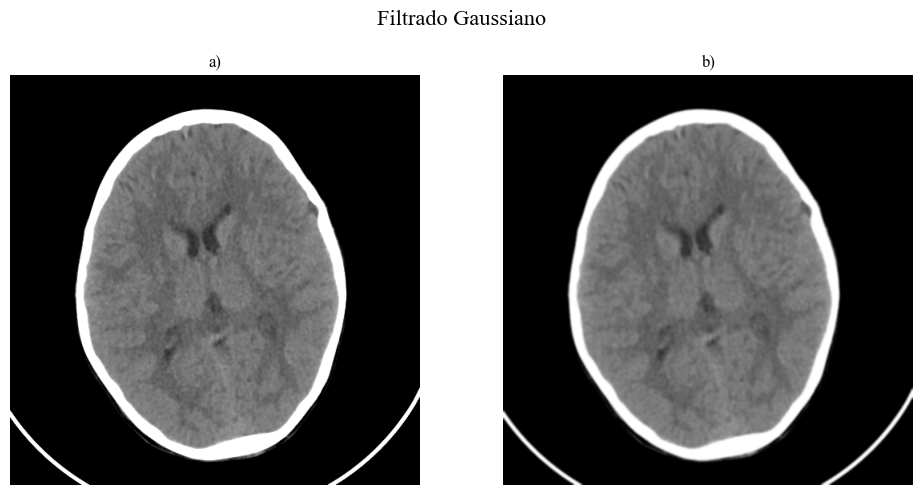
\includegraphics[width=0.95\textwidth]{Graphics/gaussian-filter.png}
    \caption{Comparación visual del efecto del filtrado gaussiano en una imagen de CT de cráneo: (a) imagen original, (b) imagen luego de la aplicación del filtro gaussiano.}
    \label{fig:filter-gaussian}
\end{figure}

\subsubsection{Filtrado de Mediana}

El filtrado de mediana es otro método ampliamente utilizado para la mejora de imágenes médicas, particularmente eficaz en la eliminación de ruido de impulso, como el conocido ``ruido sal y pimienta''. A diferencia de los filtros lineales, el filtrado de mediana es no lineal, pues reemplaza el valor de cada píxel por la mediana de los valores de intensidad de sus vecinos dentro de una ventana definida. Esta característica permite suprimir eficazmente los valores atípicos sin suavizar excesivamente los bordes ni perder detalles estructurales importantes.

Por ello, el filtrado de mediana es especialmente valorado en aplicaciones donde la preservación de las estructuras finas, como vasos sanguíneos o límites tisulares, es prioritaria. No obstante, su desempeño puede verse afectado en presencia de grandes regiones de ruido o cuando se utilizan ventanas demasiado grandes (Figura~\ref{fig:filter-median}), lo que podría conducir a la pérdida de información relevante \cite{ImageProcessingBook}.

\begin{figure}[H]
    \centering
    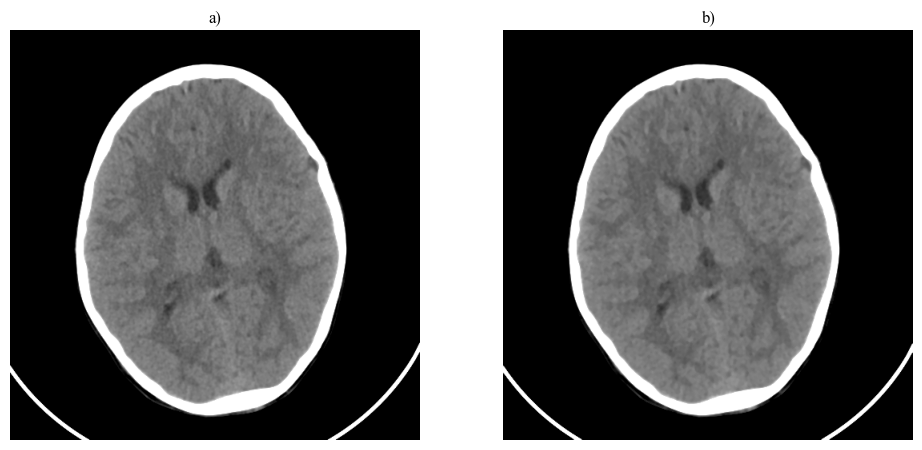
\includegraphics[width=0.95\textwidth]{Graphics/median-filter.png}
    \caption{Comparación visual del efecto del filtrado de mediana en una imagen de CT de cráneo: (a) imagen original, (b) imagen luego de la aplicación del filtro de mediana.}
    \label{fig:filter-median}
\end{figure}

\subsubsection{Ecualización Adaptativa del Histograma (CLAHE)}

La ecualización adaptativa del histograma, conocida como CLAHE (\textit{Contrast Limited Adaptive Histogram Equalization} \cite{CLAHE}), es una técnica avanzada de mejora de contraste que se utiliza ampliamente en el procesamiento de imágenes médicas \cite{CLAHE}. A diferencia de la ecualización global de histograma, que redistribuye las intensidades de toda la imagen de manera uniforme, CLAHE divide la imagen en pequeñas regiones o mosaicos y aplica la ecualización de histograma de forma local en cada uno de ellos. Este enfoque permite resaltar detalles en áreas específicas sin amplificar excesivamente el ruido ni crear artefactos indeseados, lo que resulta especialmente útil en imágenes con variaciones locales de contraste, como las obtenidas en CT.

CLAHE incorpora un parámetro de limitación de contraste (\emph{clip limit}) que controla el grado de realce permitido en cada mosaico, evitando la sobre-amplificación del ruido en regiones homogéneas. Además, el tamaño de los mosaicos (\emph{tileGridSize}) puede ajustarse para equilibrar el nivel de detalle local y el efecto global del contraste. Esta técnica ha demostrado ser eficaz para mejorar la visibilidad de estructuras sutiles en tejidos blandos o regiones con bajo contraste, facilitando el análisis y la interpretación clínica \cite{rangayyan2005biomedical}. Sin embargo, su aplicación debe realizarse con precaución, ya que un ajuste inadecuado de los parámetros puede introducir artefactos o modificar la apariencia de ciertas regiones relevantes para el diagnóstico (Figura~\ref{fig:filter-clahe}).

\begin{figure}[H]
    \centering
    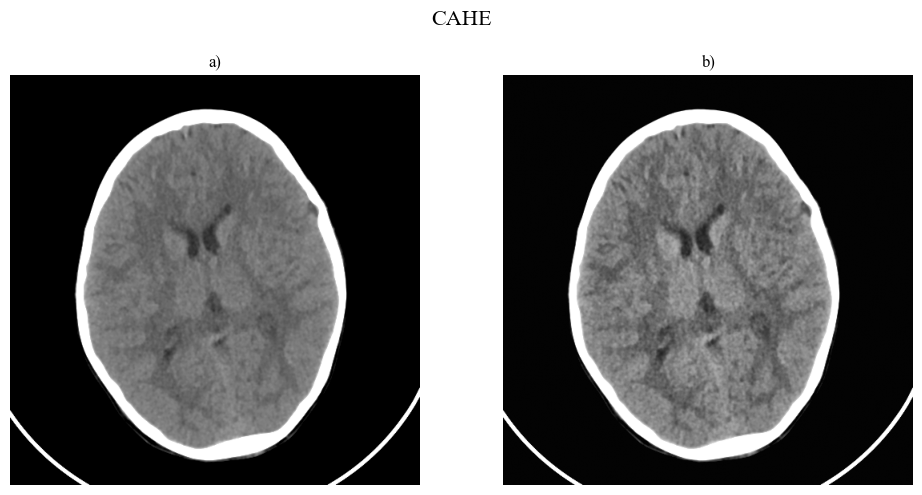
\includegraphics[width=0.95\textwidth]{Graphics/cahe.png}
    \caption{Comparación visual del efecto de la ecualización adaptativa del histograma en una imagen de CT de cráneo: (a) imagen original, (b) imagen luego de la aplicación de CLAHE.}
    \label{fig:filter-clahe}
\end{figure}

\subsubsection{Transformación Homomórfica}

La transformación homomórfica \cite{HomomorphicFilter} es un método clásico orientado a la mejora simultánea del contraste y la nitidez en imágenes digitales. Su fundamento radica en el modelado de la imagen como el producto de dos componentes: la iluminación (de baja frecuencia) y la reflectancia (de alta frecuencia). Mediante una transformación logarítmica, este producto se convierte en una suma, lo que permite la aplicación de filtros en el dominio de la frecuencia para atenuar las variaciones lentas de iluminación y realzar los detalles finos asociados a los bordes y texturas.

En el contexto de las imágenes médicas, la transformación homomórfica es especialmente útil para corregir problemas de iluminación no uniforme y para destacar estructuras anatómicas que podrían pasar desapercibidas en cortes oscuros o mal iluminados. Tras el procesamiento, se aplica la transformación exponencial inversa para reconstruir la imagen mejorada. Este método ofrece la ventaja de mejorar el contraste local y global de manera simultánea, incrementando la claridad de los bordes y la percepción de detalles relevantes para el diagnóstico. No obstante, la selección adecuada de los parámetros del filtro es crucial para evitar la introducción de artefactos y preservar la información diagnóstica esencial (Figura~\ref{fig:filter-homomorphic}).

\begin{figure}[H]
    \centering
    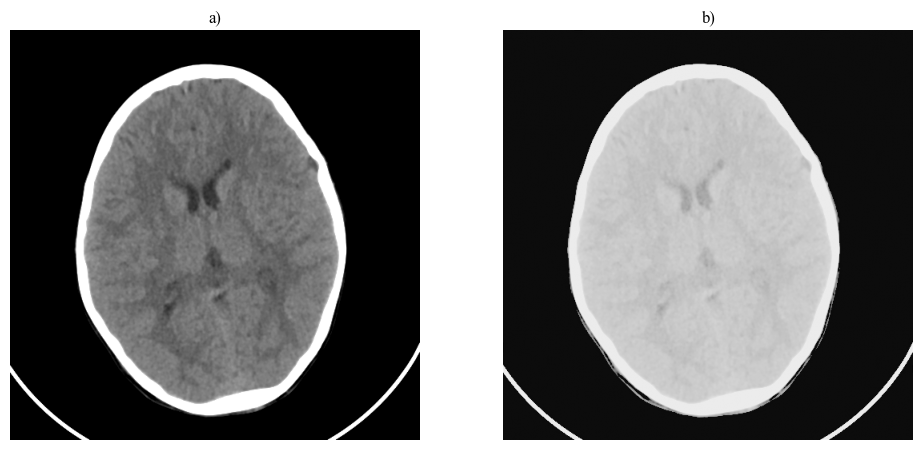
\includegraphics[width=0.95\textwidth]{Graphics/homomorphic.png}
    \caption{Comparación visual del efecto de la transformación homomórfica en una imagen de CT de cráneo: (a) imagen original, (b) imagen luego de la aplicación de la transformación homomórfica.}
    \label{fig:filter-homomorphic}
\end{figure}

\subsubsection{Detección de Bordes (Canny o laplaciano)}

La detección de bordes es una técnica fundamental en el procesamiento de imágenes médicas, cuyo objetivo principal es resaltar los contornos y límites anatómicos presentes en la imagen \cite{CannyBorderDetection,LaplacianBorderDetection}. Los métodos clásicos, como el detector de Canny y el operador laplaciano, permiten identificar transiciones abruptas de intensidad, que suelen corresponder a los bordes entre diferentes tejidos u órganos. La aplicación de estos algoritmos facilita la delimitación precisa de regiones de interés, como órganos, vasos sanguíneos o lesiones, lo que resulta esencial para tareas posteriores de segmentación, cuantificación y análisis morfológico.

El detector de Canny es capaz de localizar bordes de forma robusta y continua, minimizando la detección de falsos positivos gracias a su enfoque multietapa que incluye suavizado, cálculo de gradientes, supresión de no-máximos y umbralización con histéresis. Por otro lado, el operador laplaciano, basado en la segunda derivada de la intensidad, destaca los puntos de cambio rápido en la imagen, aunque es más sensible al ruido y suele emplearse en combinación con técnicas de suavizado previo.

En el contexto de la CT, la detección de bordes contribuye significativamente a la mejora de la visualización de estructuras anatómicas y a la precisión de los procesos de diagnóstico asistido por computadora, permitiendo una interpretación más clara y objetiva de las imágenes (Figura~\ref{fig:filter-canny}).

\begin{figure}[H]
    \centering
    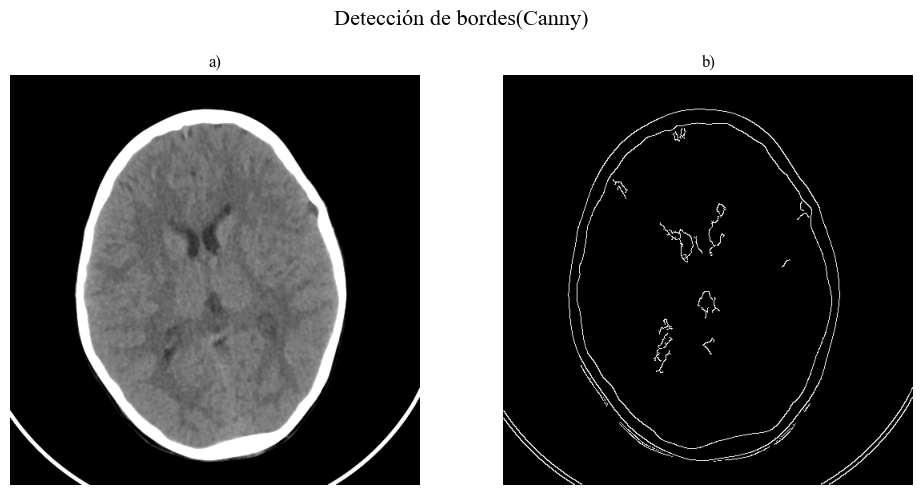
\includegraphics[width=0.95\textwidth]{Graphics/canny.png}
    \caption{Comparación visual del efecto de la detección de bordes mediante el filtro de Canny en una imagen de CT de cráneo: (a) imagen original, (b) imagen luego de la aplicación del detector de bordes Canny.}
    \label{fig:filter-canny}
\end{figure}

\subsection{Métodos basados en aprendizaje automático y profundo}

\subsubsection{EDCNN}

Uno de los avances recientes en la mejora de imágenes de CT de baja dosis es el modelo EDCNN (\textit{Edge enhancement-based Densely Connected Network} \cite{EDCNN}), una red neuronal convolucional diseñada específicamente para la reducción de ruido, manteniendo la integridad de los detalles anatómicos. EDCNN introduce un módulo de mejora de bordes que utiliza operadores Sobel entrenables para extraer y realzar características de bordes en múltiples direcciones, integrando estos mapas de bordes con la imagen original como entrada al modelo. Esta estrategia permite preservar estructuras finas y contornos, superando la tendencia al sobresuavizado observada en métodos previos.

La arquitectura de EDCNN se basa en una red convolucional con conexiones densas, inspirada en DenseNet \cite{huang2017densely}, que facilita la fusión de información jerárquica y de bordes a lo largo de la red. Además, emplea una función de pérdida compuesta que combina el error cuadrático medio (MSE) con una pérdida perceptual multi-escala basada en ResNet-50, lo que favorece la similitud tanto a nivel de píxel como de estructuras visuales. 

Los resultados reportados en el dataset NIH AAPM-Mayo Clinic LDCT \cite{moen2021low} demuestran que EDCNN logra una reducción de ruido efectiva y una mejor preservación de detalles en comparación con modelos clásicos y otros métodos de aprendizaje profundo, obteniendo altas puntuaciones en métricas cuantitativas (PSNR, SSIM) y en evaluaciones subjetivas realizadas por radiólogos.

\subsubsection{LEARN++}

Un avance relevante en el campo de la reconstrucción de imágenes de CT con sensado comprimido es el modelo LEARN++ \cite{LEARN++}. Esta arquitectura, basada en redes neuronales recurrentes de doble dominio, está diseñada para abordar los desafíos asociados a la reconstrucción a partir de un número reducido de vistas y a la reducción de la dosis de radiación.

A diferencia de métodos tradicionales y enfoques basados en un solo dominio, LEARN++ procesa simultáneamente la información en los dominios de la imagen y del sinograma, permitiendo una interacción paralela y continua entre ambos. La red integra una subred convolucional dedicada a la restauración de imágenes y otra orientada al \textit{inpainting} adaptativo de sinogramas, logrando así una mayor consistencia de datos y una mejor preservación de detalles anatómicos.

La función de pérdida compuesta de LEARN++ combina el error cuadrático medio tanto en el dominio de la imagen como en el sinograma, junto con una pérdida perceptual basada en características extraídas por VGG-19. Esta combinación permite equilibrar la fidelidad de los datos con la calidad visual y estructural de las imágenes reconstruidas. Los resultados obtenidos en el dataset NIH-AAPM-Mayo Clinic LDCT demuestran que LEARN++ supera significativamente a modelos previos en métricas cuantitativas como PSNR y SSIM, así como en evaluaciones subjetivas realizadas por radiólogos, destacándose por su capacidad para eliminar artefactos, reducir el ruido y preservar estructuras de bajo contraste.

\subsubsection{ULTRA}

El modelo ULTRA \cite{ULTRA} constituye una propuesta avanzada para la reconstrucción de imágenes en CT espectral  mediante aprendizaje profundo. Basado en una arquitectura U-Net modificada con conexiones densas y filtros multicanal, ULTRA está diseñado para fusionar información multiescala y mejorar la extracción de características relevantes en imágenes adquiridas a diferentes energías. Entre sus innovaciones destaca la introducción de una función de pérdida generalizada, que permite controlar el equilibrio entre suavizado y preservación de bordes, así como una regularización por variación total anisotrópica que aprovecha las correlaciones espaciales y espectrales entre los distintos \textit{bins} de energía.

Este enfoque aborda eficazmente los retos inherentes a la TC espectral, como la baja relación señal-ruido y la presencia de artefactos, superando las limitaciones de los métodos tradicionales basados en variación total o diccionarios tensoriales, que suelen ser computacionalmente costosos y sensibles a la selección de parámetros. ULTRA combina los beneficios del aprendizaje profundo con técnicas de regularización física, logrando una reconstrucción eficiente y precisa, con tiempos de procesamiento comparables a los métodos analíticos convencionales.

Los resultados experimentales, tanto en simulaciones como en estudios preclínicos y con maniquíes físicos, demuestran que ULTRA supera a los métodos clásicos y otras redes profundas en métricas cuantitativas y cualitativas, preservando detalles anatómicos y mejorando la descomposición de materiales.

\subsubsection{DLR}

Las técnicas de reconstrucción basadas en aprendizaje profundo (\textit{Deep Learning Reconstruction}, DLR \cite{DLR}) han emergido como una alternativa avanzada para mejorar la calidad de imagen en angiografías por CT cerebral (CTA), superando las limitaciones de los métodos tradicionales como la retroproyección filtrada (FBP) y la reconstrucción iterativa híbrida (Hybrid IR). DLR utiliza redes neuronales convolucionales entrenadas con imágenes de referencia de alta calidad para diferenciar entre señal anatómica y ruido, permitiendo una reducción significativa del ruido y los artefactos sin sacrificar la resolución espacial ni la textura natural de la imagen.

Estudios recientes han demostrado que DLR no solo mejora métricas objetivas como la relación señal-ruido (SNR) y la relación contraste-ruido (CNR), sino que también incrementa la nitidez de bordes y la visualización de vasos pequeños, aspectos críticos en el diagnóstico de patologías vasculares intracraneales. Además, DLR ofrece tiempos de reconstrucción más rápidos que los métodos iterativos basados en modelos, lo que facilita su integración en la práctica clínica diaria. Algoritmos comerciales como AiCE (Canon) y TrueFidelity™ (GE) ya cuentan con validación clínica y aprobación regulatoria, consolidando el papel del aprendizaje profundo en la reconstrucción de imágenes médicas.

En síntesis, la reconstrucción basada en aprendizaje profundo representa un avance sustancial en la calidad y eficiencia de la CTA cerebral, permitiendo una mejor visualización de estructuras vasculares complejas y una reducción de artefactos, con potencial para optimizar el diagnóstico y tratamiento de enfermedades cerebrovasculares.

\section{Propuesta}

\subsection{Transformada \textit{curvelet}}

La transformada \textit{curvelet} es una técnica de análisis multirresolución diseñada para representar de manera eficiente señales e imágenes con singularidades a lo largo de curvas suaves. A diferencia de la transformada \textit{wavelet}, que ofrece una representación óptima de singularidades puntuales, la \textit{curvelet} proporciona una representación parsimoniosa de estructuras curvilíneas y bordes en imágenes, gracias a su capacidad de adaptación direccional y anisotropía controlada \cite{Curvelets2000,FastCurveletTransform}.

\subsubsection{Fundamentos Matemáticos}

En su formulación continua, una \textit{curvelet} se define como una función de base indexada por tres parámetros: 
\begin{itemize}
    \item \textbf{Escala} (\(j \in \mathbb{N}\)): Controla el tamaño de la \textit{curvelet}.
    \item \textbf{Orientación} (\(\theta_l \in [0, 2\pi)\)): Determina la dirección principal de la curva.
    \item \textbf{Posición} (\(k \in \mathbb{Z}^2\)): Localiza la \textit{curvelet} en el espacio.
\end{itemize}

La \textit{curvelet} madre \(\phi_j(x)\) se dilata, rota y traslada para generar la familia de funciones:
\[
\phi_{j,l,k}(x) = 2^{-3j/4} \phi_j \left( R_{\theta_l}^{-1}(x - x_k^{(j,l)}) \right),
\]
donde \(R_{\theta_l}\) es la matriz de rotación y \(x_k^{(j,l)}\) denota la posición central en la escala \(j\) y orientación \(\theta_l\).

En el dominio de Fourier, las curvelets se localizan en regiones en forma de cuña, con soporte anisotrópico que satisface la relación:
\[
\text{Ancho} \sim 2^{-j/2}, \quad \text{Largo} \sim 2^{-j}.
\]

\subsubsection{Transformada Curvelet Discreta}

La implementación discreta se realiza en el dominio de Fourier mediante los siguientes pasos \cite{FastCurveletTransform}:
\begin{enumerate}
    \item Aplicar la transformada de Fourier bidimensional (2D FFT) a la imagen.
    \item Multiplicar el espectro por ventanas angulares \(U_{j,l}(\omega)\) que aíslan bandas de frecuencia y dirección.
    \item Reorganizar (\emph{wrapping}) cada cuña espectral en un rectángulo centrado en el origen.
    \item Aplicar la transformada inversa de Fourier (2D IFFT) para obtener los coeficientes \textit{curvelet} \(c(j,l,k)\).
\end{enumerate}

Matemáticamente, los coeficientes se calculan como:
\[
c(j,l,k) = \frac{1}{(2\pi)^2} \int_{\mathbb{R}^2} \hat{f}(\omega) U_{j,l}(\omega) e^{i\langle x_k^{(j,l)}, \omega \rangle} d\omega,
\]
donde \(\hat{f}(\omega)\) es el espectro de la imagen original.

\subsubsection{Ventajas sobre Otras Transformadas}

\begin{figure}[H]
    \centering
    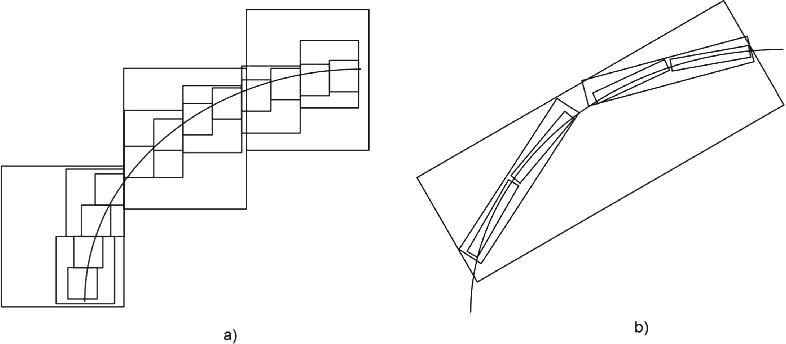
\includegraphics[width=0.95\textwidth]{Graphics/Comparison-between-approximation-using-a-wavelet-and-b-curvelet-12.png}
    \caption{Comparación visual entre la aproximación: (a) usando \textit{wavelets}, (b) usando \textit{curvelets}. \cite{comparison}}
    \label{fig:comparison-wavelet-curvelet}
\end{figure}

La \textit{curvelet} supera a la \textit{wavelet} en dos aspectos clave:
\begin{itemize}
    \item \textbf{Sensibilidad direccional}: Detecta bordes y curvas en múltiples orientaciones (Figura~\ref{fig:comparison-wavelet-curvelet}).
    \item \textbf{Representación esparsa}: Requiere menos coeficientes para representar edges, reduciendo redundancia.
\end{itemize}

Estas propiedades la hacen ideal para aplicaciones en imágenes médicas, donde la preservación de bordes anatómicos y la supresión de ruido son críticas.

\subsection{Transformada \textit{Synchrosqueezed Curvelet}}

La transformada \textit{synchrosqueezed curvelet} (SSCT, por sus siglas en inglés) es una técnica avanzada de post-procesamiento que combina la capacidad direccional de la transformada \textit{curvelet} con un método de reasignación espectral para lograr una representación más precisa de componentes modales en imágenes. Este enfoque es particularmente efectivo para analizar señales bidimensionales con frentes de onda curvos o componentes de banda estrecha, donde los métodos tradicionales fallan en separar modos superpuestos \cite{SynchrosqueezedCurveletTransform}.

\subsubsection{Principios Fundamentales}

La SSCT opera en dos etapas principales:
\begin{enumerate}
    \item \textbf{Transformada Curvelet Generalizada}: Aplica una transformada \textit{curvelet} con parámetros de escalado geométrico adaptativos (escala radial \(t\) y angular \(s\)) para capturar componentes direccionales.
    \item \textbf{Reasignación espectral (\textit{synchrosqueezing})}: Reubica los coeficientes \textit{curvelet} en el espacio fase, basándose en estimaciones precisas de vectores de onda locales, condensando la energía en regiones más compactas.
\end{enumerate}

\subsubsection{Formulación Matemática}

Dada una imagen \(f(x)\), la SSCT se define mediante:
\begin{itemize}
    \item \textbf{Transformada \textit{curvelet}}: 
    \[
    W_f(a, \theta, b) = \langle f, \phi_{a,\theta,b} \rangle = \int_{\mathbb{R}^2} f(x) \overline{\phi_{a,\theta,b}(x)} dx,
    \]
    donde \(\phi_{a,\theta,b}(x)\) son las curvelets con escala \(a\), orientación \(\theta\) y posición \(b\).
    
    \item \textbf{Estimación del Vector de Onda Local}:
    \[
    v_f(a, \theta, b) = \frac{\nabla_b \arg(W_f(a, \theta, b))}{2\pi}.
    \]
    Este operador de fase estima la frecuencia instantánea en la dirección dominante.
    
    \item \textbf{Reasignación}:
    Los coeficientes se reubican según:
    \[
    T_f(v, b) = \int_{A(v, b)} W_f(a, \theta, b) a^{-3/2} da d\theta,
    \]
    donde \(A(v, b) = \{(a, \theta): v_f(a, \theta, b) = v\}\) agrupa coeficientes con el mismo vector de onda estimado \cite{SynchrosqueezedCurveletTransform}.
\end{itemize}

\subsubsection{Ventajas}

El \textit{synchrosqueezing} aplicado a la transformada \textit{curvelet} ofrece varias ventajas clave en el análisis y descomposición de señales bidimensionales. En primer lugar, permite una \textbf{resolución mejorada} al reducir la dispersión espectral de los coeficientes \textit{curvelet}, lo que se traduce en representaciones más nítidas y precisas de las estructuras presentes en la señal, como se observa en la Figura 2. 

Además, esta técnica facilita la \textbf{separación de modos} en señales compuestas, ya que, para funciones de la forma \( f(x) = \sum_k f_k(x) \) cuyos vectores de onda están bien separados \(\left|\nabla \phi_k - \nabla \phi_l\right| \geq d\), la Synchrosqueezed Curvelet Transform (SSCT) permite identificar cada componente \( f_k \) mediante algoritmos de \textit{clustering} en el espacio de fase reasignado.

Por otra parte, la SSCT presenta \textbf{invariancia a la curvatura}, lo que la distingue de los métodos basados en \textit{wavelets} tradicionales. Gracias a la anisotropía inherente de las \textit{curvelets}, esta técnica preserva de manera eficiente la estructura de los componentes curvilíneos, manteniendo la fidelidad de las formas presentes en la señal original.

\subsubsection{Aplicación en Procesamiento de Imágenes Médicas}

En el contexto de tomografías de cráneo, la Synchrosqueezed Curvelet Transform (SSCT) ofrece ventajas relevantes para el procesamiento avanzado de imágenes médicas. En primer lugar, permite mejorar el contraste mediante la separación espectral de tejidos con diferentes propiedades de atenuación, facilitando la distinción de estructuras anatómicas sutiles. Además, contribuye a la reducción de artefactos de ``blooming'' en presencia de estructuras metálicas, gracias a la reasignación selectiva de coeficientes en el dominio espectral. Por último, la SSCT posibilita la cuantificación de texturas anatómicas a través del análisis de mapas de vectores de onda locales, lo que resulta útil para la caracterización detallada de patrones tisulares en las imágenes de tomografía computarizada de cráneo.

\subsection{Propuesta Metodológica}

La propuesta desarrollada en esta tesis consiste en la aplicación de la transformada SSCT a imágenes de CT del cerebro. El procedimiento se inicia con la descomposición de la imagen original mediante la SSCT, obteniendo así una representación espectral detallada en el dominio espacio-frecuencia, capaz de capturar tanto las singularidades direccionales como la información multiescala inherente a las estructuras anatómicas cerebrales. Posteriormente, los coeficientes obtenidos a través de la SSCT son modificados mediante una función de procesamiento adecuada, diseñada para realzar las características de interés (como bordes o texturas) o atenuar componentes indeseados (como ruido o artefactos). Finalmente, se reconstruye la imagen a partir de los coeficientes modificados, generando una versión mejorada que se espera presente mayor calidad diagnóstica, con mejor contraste y preservación de detalles relevantes.

Cabe destacar que esta metodología es de naturaleza numérica pura y no depende de técnicas de inteligencia artificial ni de aprendizaje profundo. A diferencia de los métodos basados en redes neuronales, que han demostrado excelentes resultados en la mejora de imágenes médicas pero requieren grandes volúmenes de datos etiquetados, conocimien

\subsubsection{Umbralización}

El método de umbralización consiste en aplicar un umbral fijo a la energía obtenida por la SSCT, de modo que sólo se conserven los valores superiores a un cierto nivel predefinido. Este procedimiento es ampliamente utilizado en el procesamiento de imágenes médicas para segmentar regiones de interés o eliminar componentes de bajo valor energético, facilitando la extracción de estructuras relevantes \cite{zhao2023thresholding, pmc6132127}. La elección del valor de umbral es un parámetro crítico, ya que determina el equilibrio entre la preservación de detalles y la supresión de ruido o artefactos.

\subsubsection{Potenciación de la Energía SSCT}

La potenciación de la energía SSCT consiste en modificar los valores obtenidos de la transformada elevando la energía a una potencia específica (parámetro de enhancement). Esta operación no lineal permite realzar selectivamente las diferencias entre regiones de alta y baja energía, incrementando el contraste local y facilitando la discriminación de estructuras anatómicas sutiles. Los métodos de potenciación y manipulación no lineal de coeficientes han sido explorados en el contexto de transformadas multiescala para el realce de imágenes médicas, mostrando mejoras en la percepción visual y en métricas objetivas de calidad \cite{SynchrosqueezedCurveletTransform, EnergyEnhancement}.

\subsubsection{Enmascaramiento del Resultado de la Transformada SSCT}

El enmascaramiento consiste en aplicar una máscara binaria o ponderada sobre el dominio SSCT, permitiendo conservar únicamente aquellas regiones que cumplen ciertos criterios (por ejemplo, localización anatómica, dirección predominante o magnitud de energía). Esta técnica es útil para focalizar el procesamiento en áreas de interés clínico y reducir la influencia de regiones irrelevantes o ruidosas.

El enmascaramiento en el dominio de transformadas ha sido utilizado para mejorar la segmentación y el análisis de imágenes médicas, optimizando la relación señal-ruido y la especificidad de los resultados \cite{SynchrosqueezedCurveletTransform,ImageMaskingBook}.

\vspace{0.5cm}

En síntesis, la propuesta metodológica se fundamenta en el uso de herramientas matemáticas robustas y eficientes para el procesamiento de imágenes médicas, ofreciendo una alternativa viable y accesible para la mejora de la calidad de imágenes de CT cerebral en entornos con restricciones tecnológicas y de recursos humanos.

% \include{MainMatter/Proposal}
% \chapter{Detalles de Implementación y Experimentos}\label{chapter:implementation}

En este capítulo se describe detalladamente el proceso de implementación del método propuesto para la mejora de imágenes de tomografía computarizada cerebral. Se presentan las herramientas y entornos de desarrollo empleados, así como las adaptaciones realizadas sobre las implementaciones existentes de la transformada synchrosqueezed (SST) y su inversa (ISST) en el contexto de la transformada curvelet bidimensional (2DCT). Además, se explican los procedimientos seguidos para el preprocesamiento de los datos, la configuración de los experimentos y la aplicación de las distintas estrategias de modificación de la matriz de energía. Finalmente, se justifica la selección de los parámetros experimentales y se expone la estructura general del flujo de trabajo, sentando las bases para la posterior evaluación y comparación de los resultados obtenidos.

\section{Ambiente de trabajo y herramientas}\label{section:work-environment}

El funcionamiento principal de los experimentos gira alrededor de la implementación original de las funciones de SST e ISST, por Haizhao Yang y Lexing Ying \cite{SynchrosqueezedCurveletTransform_SynLab}. Esta fue originalmente concebida en \texttt{Matlab}, un software y lenguaje de programación matemático, con gran énfasis en la practicidad y en la facilidad de uso para personal del sector científico. Esta implementación, con cambios mínimos, fue exportada a \texttt{GNU Octave}, una versión gratuita y de código abierto creada y mantenida por una extensa comunidad de contribuidores. Esto se hizo con el objetivo de poder utilizarlo sin la restricción de las barreras de pago, que en nuestro país se hace de gran dificultad. Esta implementación se encuentra modularizada en el repositorio de la tesis.

Dada la elevada dificultad de la implementación de SST y de ISST, además de la complejidad para crear experimentos complejos y paralelizables para mejor rendimiento, esta fue usada solo como una librería dinámica la cual fue llamada desde \texttt{Python 3.13}. Para esto, se usó la librería \texttt{oct2py}, la cual permite integración directa con el motor de \texttt{Octave} para llamar a las funciones definidas (en este caso solo SST e ISST) con objetos nativos de \texttt{Python}, como son arreglos n-dimensionales de \texttt{numpy}.

Durante el desarrollo y la ejecución de los experimentos, el código fue implementado y ejecutado íntegramente en la unidad central de procesamiento (CPU) de un equipo portátil de alto rendimiento. Este sistema cuenta con un procesador AMD Ryzen 7 8845HS de 8 núcleos y 16 hilos, con una frecuencia base de 3.8 GHz y una frecuencia máxima de hasta 5.1 GHz. Además, dispone de 32 GB de memoria RAM DDR5 y una unidad de almacenamiento sólido (SSD) de 1 TB. Todas las tareas de procesamiento, incluidas las etapas más intensivas computacionalmente, se realizaron exclusivamente en la CPU, sin recurrir a aceleración por hardware gráfico. Estas especificaciones proporcionaron un entorno adecuado para evaluar el rendimiento y la escalabilidad de la implementación propuesta, asegurando resultados reproducibles y tiempos de ejecución competitivos.

Adicionalmente, para el manejo, procesamiento y análisis de los resultados, se emplearon diversas herramientas del ecosistema científico de Python, tales como \texttt{numpy} para operaciones matriciales y de álgebra lineal, \texttt{matplotlib} para la visualización de datos y \texttt{pandas} para la manipulación de conjuntos de datos. El desarrollo de scripts experimentales, automatización de pruebas y gestión de resultados se realizó en un entorno de desarrollo basado en \texttt{Jupyter Notebook}, lo que facilitó la documentación interactiva y la reproducibilidad de los experimentos. Para el control de versiones y la colaboración, se utilizó el sistema \texttt{git}, permitiendo un seguimiento detallado de los cambios y la integración eficiente de mejoras en el código fuente. Finalmente, la ejecución de los experimentos se gestionó mediante scripts de automatización en \texttt{bash} y el uso de entornos virtuales con \texttt{conda} para asegurar la compatibilidad y portabilidad de las dependencias empleadas a lo largo del proyecto.

Para garantizar la reproducibilidad de los resultados y la consistencia en los experimentos, se fijaron explícitamente las semillas aleatorias y las configuraciones relevantes en todos los procesos. Esto permitió obtener resultados comparables y facilitar la validación de los procedimientos implementados.

\section{Optimización de la implementación}\label{section:optimization}

Con el objetivo de mejorar la eficiencia y el rendimiento de la solución propuesta, se han incorporado las siguientes optimizaciones en la implementación:

\begin{itemize}
    \item \textbf{Caché de los datos obtenidos:} Se ha implementado un sistema de almacenamiento temporal de los datos intermedios, como son el resultado de aplicar SST sobre una imagen en particular. Esta estrategia permite reutilizar resultados previamente calculados y reducir el acceso a la memoria principal o la necesidad de recomputar información, lo que se traduce en una disminución significativa del tiempo de ejecución global.
    
    \item \textbf{Paralelización de la ejecución:} Se ha aprovechado la capacidad de procesamiento concurrente de \texttt{Python} mediante la paralelización del procesamiento de imágenes independientes. Esto permite distribuir la carga de trabajo entre múltiples núcleos o hilos, acelerando etapas críticas como el cálculo de transformadas y la reconstrucción de imágenes, y logrando una mejora sustancial en los tiempos de cómputo.
    
    \item \textbf{Limpieza de los objetos no utilizados en memoria:} Para evitar la acumulación innecesaria de datos y prevenir posibles fugas de memoria, se ha incorporado un mecanismo de liberación sistemática de los objetos que ya no son requeridos durante la ejecución. Esta gestión eficiente de la memoria contribuye a mantener la estabilidad y el rendimiento de la aplicación, especialmente en experimentos de gran escala o en entornos con recursos limitados.
\end{itemize}

La necesidad de implementar optimizaciones en el procesamiento de imágenes surge de las exigencias computacionales observadas durante el desarrollo experimental. En primer lugar, el resultado de la SST aplicada a una sola imagen puede ocupar aproximadamente 1.4 GB de espacio en memoria, lo que representa una carga significativa para los recursos del sistema. Además, los tiempos de ejecución para el procesamiento completo de una imagen —incluyendo tanto la SST como su inversa (ISST)— alcanzan una media de 4 minutos, lo que limita la viabilidad del método en escenarios donde se requiere el análisis de grandes volúmenes de datos o la respuesta en tiempo real. Por otro lado, el consumo de memoria RAM sin la aplicación de optimizaciones puede llegar a ser muy intenso, alcanzando picos de hasta 15 GB durante la ejecución de múltiples experimentos. Estas condiciones motivan la incorporación de técnicas específicas de optimización, orientadas a reducir el uso de memoria, agilizar los tiempos de procesamiento y garantizar la estabilidad del sistema, permitiendo así la aplicación práctica y eficiente del método propuesto en entornos computacionales con recursos limitados.

Como resultado de las optimizaciones implementadas, se logró una reducción significativa tanto en los tiempos de ejecución como en el consumo de memoria del sistema. Tras la aplicación de estas mejoras, el tiempo medio de procesamiento por experimento —incluyendo la aplicación de SST e ISST sobre una imagen— disminuyó a aproximadamente 2 minutos, lo que representa una mejora sustancial en la eficiencia operativa del método. Asimismo, el uso máximo de memoria RAM durante la ejecución se redujo a 4 GB, permitiendo la realización de experimentos en equipos con recursos más limitados y mejorando la estabilidad general del sistema durante la ejecución de múltiples tareas en paralelo. Estos resultados evidencian la efectividad de las estrategias de optimización adoptadas en el desarrollo de la presente implementación.

\section{Implementación de los experimentos} \label{section:experiment-implementation}

La implementación de los experimentos se basa en un flujo modular que permite el procesamiento eficiente y reproducible de imágenes. El proceso inicia con la carga y normalización de las imágenes, que pueden provenir tanto de archivos individuales en formatos estándar (\texttt{.jpg} o \texttt{png}) como de volúmenes médicos (\texttt{.nii}). Para la gestión y muestreo de imágenes, se emplean objetos utilitarios que permiten recuperar conjuntos de imágenes desde directorios estructurados, facilitando la selección aleatoria o secuencial de muestras para los experimentos.

En cuanto al preprocesamiento, este se aplicó de manera diferenciada según la naturaleza de los experimentos. En una primera serie de experimentos, las imágenes fueron normalizadas para que sus valores de intensidad se encontraran en el rango $[0, 1]$. Esta normalización permitió asegurar la homogeneidad en la escala de entrada y facilitó la comparación directa entre diferentes muestras, independientemente de su origen o condiciones de adquisición.

En una segunda serie de experimentos, se utilizaron imágenes volumétricas en formato \texttt{.nii}, sobre las cuales se aplicó una ventana de intensidad específica para procesar únicamente la sección correspondiente a la densidad del cerebro. Esta técnica de ventana permitió resaltar las estructuras anatómicas de interés y reducir el impacto de regiones irrelevantes o valores atípicos, optimizando así la calidad y relevancia de los datos utilizados en el análisis posterior.

Cabe destacar que la naturaleza del preprocesamiento aplicado influyó notablemente en los tiempos de ejecución de los experimentos. En la primera serie, al trabajar con imágenes normalizadas en un rango reducido de valores, los tiempos de procesamiento fueron considerablemente menores, con una media aproximada de 1 minuto por experimento. En contraste, la segunda serie, basada en imágenes volumétricas procesadas mediante la aplicación de una ventana de intensidad, presentó tiempos de ejecución significativamente mayores, oscilando entre 3 y 5 minutos por experimento. Esta diferencia en el rendimiento también tuvo implicaciones directas en los resultados obtenidos, las cuales serán analizadas en detalle en una sección posterior.% todo

Una vez cargadas y preprocesadas, las imágenes son transformadas mediante la aplicación de la transformada synchrosqueezed curvelet y su inversa. Este procedimiento se encuentra encapsulado en objetos que gestionan tanto la ejecución de las transformadas como la utilización de un sistema de caché, el cual almacena los resultados intermedios para evitar recomputaciones innecesarias y optimizar el uso de recursos. Los resultados de la transformada se almacenan en estructuras especializadas que contienen la energía synchrosqueezed, los coeficientes curvelet y los vectores asociados, permitiendo su manipulación eficiente en las siguientes etapas del experimento.

Las funciones experimentales, están implementadas como procedimientos puros que operan sobre los resultados de la transformada, generando nuevas instancias modificadas de dichos resultados sin alterar los datos originales. La ejecución de cada experimento se gestiona a través de utilidades que reciben una configuración detallada, especificando la función experimental a aplicar, los parámetros y los argumentos adicionales requeridos. Tras la aplicación de la función experimental, se realiza la reconstrucción de la imagen modificada mediante la transformada inversa, asegurando la consistencia del flujo de procesamiento.

Durante todo el proceso, se implementa un sistema de registro para el seguimiento detallado de cada etapa y la gestión de errores. Además, se asegura la reproducibilidad de los experimentos mediante la fijación de semillas aleatorias y la serialización de los resultados y configuraciones empleadas. Este enfoque modular y estructurado permite realizar experimentos complejos de manera eficiente, garantizando la trazabilidad y la robustez de los resultados obtenidos.

El flujo completo de procesamiento experimental se organiza a través de una función principal que recibe como entrada un conjunto de imágenes, las configuraciones específicas de los experimentos a realizar y las configuraciones de las métricas de evaluación. Internamente, esta función itera sobre cada imagen y, para cada una, aplica de manera secuencial las distintas configuraciones experimentales definidas. Para cada combinación de imagen y configuración experimental, se ejecuta el procesamiento correspondiente: primero se realiza la transformada synchrosqueezed sobre la imagen, luego se aplica la función experimental seleccionada sobre los resultados de la transformada, y finalmente se reconstruye la imagen modificada mediante la transformada inversa.

Durante este proceso, se calculan las métricas de evaluación especificadas, comparando la imagen reconstruida con la original u otras referencias según corresponda. Todos los resultados, así como los parámetros y configuraciones utilizados, se almacenan y registran de forma estructurada para su posterior análisis. Este proceso automatizado permite ejecutar grandes volúmenes de experimentos de manera eficiente, garantizando la trazabilidad y la reproducibilidad (ver imagen \ref{fig:diagrama-flujo-experimentos}).

\begin{figure}[H]
    \centering
    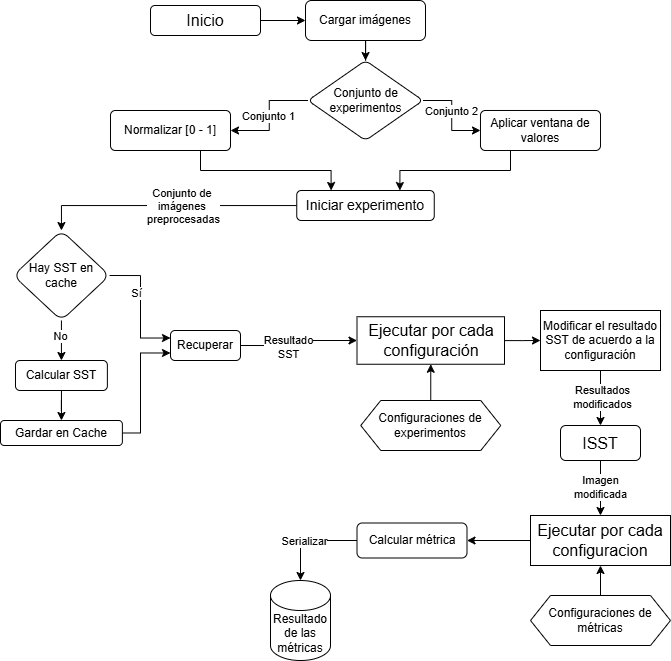
\includegraphics[width=0.95\textwidth]{Graphics/diagrama experimentos tesis.drawio.png}
    \caption{Diagrama de flujo del pipeline experimental implementado para el procesamiento y análisis de imágenes.}
    \label{fig:diagrama-flujo-experimentos}
\end{figure}

\begin{table}[h]
    \centering
    \caption{Configuraciones experimentales y sus parámetros.\cite{ExperimentSource,ExperimentSource2}}
    \label{tab:experimentos}
    \begin{tabular}{>{\raggedright}p{4cm}p{6cm}}
    \toprule
    \textbf{Tipo de Experimento} & \textbf{Parámetros} \\ 
    \midrule
    Umbralizado & threshold = 0.1, 0.05, 0.001 \\
    \midrule
    Mejora de energía & \texttt{enhancement\_factor} = 3.0, 1.5, 10 \\
    \midrule
    Filtro pasa-alto & \texttt{cutoff\_scale} = 5, 10 \\
    \midrule
    Filtro pasa-banda & \texttt{low\_scale} = 5 (\texttt{high\_scale} = 10), 15 (20) \\
    \midrule
    Máscara gaussiana & $ \mu  = N/2$, $ \sigma $ = 1.0, 4.0, 6.0 \\
    \midrule
    Máscara exponencial & \texttt{decay\_rate} = 0.1, 0.01 \\
    \bottomrule
    \end{tabular}
    \footnotesize{\\*N/2: mitad de las escalas disponibles en la descomposición.}
\end{table}

Para la realización de los experimentos se utilizó un conjunto de configuraciones específicas, las cuales se detallan en la Tabla~\ref{tab:experimentos}. Cada configuración define los parámetros y valores empleados en las distintas funciones experimentales aplicadas durante el procesamiento, permitiendo así evaluar el comportamiento del método bajo diferentes condiciones y ajustes. Esta variedad de configuraciones facilita un análisis exhaustivo y comparativo de los resultados obtenidos.

\section{Implementación de las métricas} \label{section:metrics-implementation}

Las métricas utilizadas para la evaluación cuantitativa de los resultados experimentales fueron implementadas de manera modular y eficiente, empleando herramientas especializadas del ecosistema científico de \texttt{Python}. Las configuraciones específicas de las métricas se encuentran detalladas en la Tabla~\ref{tab:metricas}

Para las métricas basadas en operaciones numéricas y estadísticas, como el índice de mejora de contraste y la razón de nitidez basada en el operador Laplaciano, se utilizó la biblioteca \texttt{numpy} para el cálculo vectorizado de desviaciones estándar y varianzas, así como \texttt{opencv-python} para la aplicación de operadores de filtrado espacial.

Las métricas perceptuales avanzadas, como el FSIM (Feature Similarity Index) y LPIPS (Learned Perceptual Image Patch Similarity), se implementaron a través de las bibliotecas \texttt{piq} y \texttt{lpips}, respectivamente, haciendo uso de \texttt{PyTorch} para el manejo de tensores y la ejecución eficiente en CPU. El índice de similitud estructural (SSIM) y la relación señal-ruido pico (PSNR) se calcularon utilizando las funciones \texttt{structural\_similarity} y \texttt{peak\_signal\_noise\_ratio} de la biblioteca \texttt{scikit-image}. Para la métrica BRISQUE, orientada a la evaluación de artefactos y ruido perceptual, se empleó la implementación disponible en \texttt{piq}.

El flujo de cálculo de métricas se integra al final de cada experimento: una vez reconstruida la imagen modificada, se aplican de forma automática todas las métricas relevantes, comparando la imagen procesada con la original o con una referencia apropiada (en este caso, con la imagen original). Cada función de métrica está desacoplada del resto del procesamiento y recibe como entrada los arreglos de imagen en formato \texttt{numpy}, asegurando así su reutilización y extensibilidad.

Los resultados de cada métrica, junto con la configuración experimental correspondiente, son almacenados y registrados de forma estructurada al finalizar cada experimento. Este enfoque garantiza la trazabilidad y facilita el análisis comparativo entre diferentes configuraciones y tipos de preprocesamiento. Además, la modularidad de la implementación permite la fácil incorporación de nuevas métricas en futuras extensiones del trabajo.

De manera concreta, para cada imagen procesada, una vez ejecutados todos los experimentos definidos, se calculan de forma automática todas las métricas seleccionadas para cada resultado. Posteriormente, los valores obtenidos de las métricas, junto con la información sobre la imagen y la configuración experimental utilizada, son serializados y almacenados en un archivo en formato \texttt{json}. Esta estrategia permite centralizar y organizar los datos de evaluación, facilitando su análisis posterior, la comparación sistemática entre diferentes métodos y la integración con herramientas externas de análisis estadístico o visualización.

\begin{table}[h]
    \centering
    \caption{Métricas de evaluación agrupadas por categorías\cite{Metrics}}
    \label{tab:metricas}
    \begin{tabular}{p{3cm}p{8cm}p{3cm}}
    \toprule
    \textbf{Categoría} & \textbf{Métrica} & \textbf{Descripción} \\ 
    \midrule
    \multirow{3}{*}{Mejora} 
    & CII (\textit{Contrast Improvement Index}) & Índice de mejora de contraste \\
    & LSR (\textit{Laplacian Sharpness Ratio}) & Cociente de nitidez Laplaciana \\
    & FSIM (\textit{Feature Similarity Index}) & Similaridad de características \\
    \midrule

    \multirow{3}{*}{Distorsión}
    & PSNR (\textit{Peak Signal-to-Noise Ratio}) & Relación señal-ruido \\
    & SSIM (\textit{Structural Similarity Index}) & Similaridad estructural \\
    & LPIPS (\textit{Learned Perceptual Image Patch Similarity}) & Similaridad perceptual \\
    \midrule

    \multirow{2}{*}{Artefactos}
    & RNS (Residual Noise Standard Deviation) & Desviación estándar del ruido residual \\
    & BRISQUE (Blind/Referenceless Image Spatial Quality Evaluator \cite{BRISQUE}) & Evaluador ciego de calidad \\
    \bottomrule
    \end{tabular}
\end{table}

\section{Implementación de las estadísticas}\label{section:statistics-implementation}

El análisis estadístico de los resultados experimentales se diseñó para comparar de manera rigurosa el desempeño de los distintos métodos evaluados. Para cada par de experimentos a comparar, se recopilaron los valores obtenidos de las métricas correspondientes en todas las imágenes procesadas. El primer paso consistió en la aplicación de pruebas de normalidad sobre la distribución de cada métrica, con el objetivo de determinar el tipo de análisis estadístico adecuado para la comparación. Las pruebas de normalidad empleadas incluyeron, entre otras, la prueba de Shapiro-Wilk.

En función de los resultados de la prueba de normalidad, se seleccionó el método estadístico más apropiado para la comparación de los dos grupos experimentales. Cuando la distribución de las métricas fue compatible con la normalidad, se utilizó la prueba t de Student para muestras independientes, permitiendo evaluar si existían diferencias estadísticamente significativas entre las medias de los grupos. En caso contrario, es decir, si la distribución no era normal, se recurrió a pruebas no paramétricas como la prueba de Mann-Whitney U, que permite comparar la mediana de dos muestras independientes sin asumir normalidad.

Si el análisis estadístico indicó que existían diferencias significativas entre los experimentos comparados, se procedió a comparar sus medias y desviaciones estándar para cada métrica, determinando así cuál de los dos experimentos presentaba un mejor desempeño según los valores observados. En caso de que no se detectaran diferencias estadísticamente significativas, se asumió que ambos experimentos ofrecían resultados equivalentes para la métrica analizada.

\begin{table}[h]
    \centering
    \caption{Resumen de las métricas utilizadas, sus valores ideales y rangos de referencia.}
    \label{tab:metrics-expected-values}
    \begin{tabular}{>{\raggedright}p{5cm}p{3cm}p{3cm}}
        \toprule
        \textbf{Métrica} & \textbf{Valor ideal} & \textbf{Rango} \\
        \midrule
        Índice de mejora de contraste (CII) & $>1$ & $[0, \infty)$ \\
        Razón laplaciana & $>1$ & $[0, \infty)$ \\
        FSIM & $1$ & $[0, 1]$ \\
        PSNR & $\infty$ & $[0, \infty)$ \\
        SSIM & $1$ & $[0, 1]$ \\
        LPIPS & $0$ & $[0, 1]$ \\
        Desviación estándar del ruido residual & $0$ & $[0, \infty)$ \\
        BRISQUE & $0$ & $[0, 100]$ \\
        \bottomrule
    \end{tabular}
\end{table}

Adicionalmente, para cada métrica se consultó una tabla de valores esperados o ideales (Tabla~\ref{tab:metrics-expected-values}), lo que permitió contextualizar los resultados obtenidos y seleccionar el experimento más favorable dentro de cada par comparado. En este proceso, se otorgó un peso mayor a aquellas métricas consideradas prioritarias para la calidad de la imagen, como el índice de similitud estructural (SSIM), que evalúa la preservación de la estructura, y la métrica de nitidez basada en el operador Laplaciano, que prioriza la definición de bordes. Esta ponderación permitió orientar la selección final hacia los experimentos que maximizan la fidelidad estructural y la nitidez en las imágenes reconstruidas.

Para el análisis estadístico de los resultados experimentales se emplearon principalmente las bibliotecas \texttt{pandas} para la manipulación y análisis de los datos tabulados, y \texttt{scipy.stats} para la ejecución de pruebas estadísticas como el test de normalidad y las pruebas de comparación entre grupos. Adicionalmente, las bibliotecas \texttt{seaborn} y \texttt{matplotlib.pyplot} se utilizaron para la visualización gráfica de los resultados y la exploración de tendencias y distribuciones. Estas herramientas permitieron realizar un análisis estadístico riguroso, reproducible y visualmente comprensible de los datos obtenidos en los experimentos.


\backmatter

% \begin{conclusions}
    El presente trabajo de diploma tuvo como objetivo general desarrollar un método numérico basado en la transformada Synchrosqueezed aplicada a Curvelets (SST-2DCT) para el mejoramiento del contraste en imágenes de tomografía computarizada (CT) de cráneo, con especial énfasis en la visualización de tejidos blandos y lesiones pequeñas sin necesidad de utilizar agentes de contraste radiológico. Este enfoque se planteó como una alternativa viable en contextos con restricciones de recursos computacionales y limitaciones en el acceso a grandes volúmenes de datos etiquetados, como es el caso del sistema de salud cubano.

    \bigskip

    A continuación, se exponen las principales conclusiones obtenidas, organizadas en correspondencia con los objetivos específicos propuestos:

    \begin{enumerate}
        \item \textbf{Implementación de la transformada SST-2DCT e ISST en Python 3.13:} Se logró desarrollar una implementación funcional y eficiente de la transformada Synchrosqueezed Curvelet y su inversa, adaptando herramientas de Octave mediante la interfaz \textit{oct2py}. Esta integración permitió la manipulación directa de imágenes en formato NIfTI y facilitó la ejecución de experimentos complejos en entornos de cómputo de propósito general.

        \item \textbf{Diseño y ejecución de experimentos de mejora de características de imagen:} Se llevaron a cabo múltiples experimentos que aplicaron diferentes estrategias de modificación sobre la matriz de energía SST, tales como potenciación, umbralización y enmascaramiento. Entre todas las variantes evaluadas, la técnica basada en \textbf{Máscara Gaussiana con parámetros $\mu = N/2$ y $\delta = 1$} resultó ser la más adecuada, al lograr un equilibrio favorable entre el realce de estructuras anatómicas sutiles y la preservación de la calidad global de la imagen.

        \item \textbf{Evaluación cuantitativa mediante métricas objetivas:} Los resultados fueron evaluados utilizando un conjunto de métricas agrupadas en tres categorías: mejora de contraste (CII, LSR, FSIM), distorsión (PSNR, SSIM, LPIPS) y detección de artefactos (RNS, BRISQUE). La \textbf{Máscara Gaussiana seleccionada} demostró un desempeño superior en la mejora del contraste y la definición de bordes sin introducir distorsiones o artefactos visuales significativos, manteniendo la integridad estructural de las imágenes.

        \item \textbf{Comparación con métodos clásicos y modernos de mejoramiento de imágenes:} La solución propuesta mostró resultados competitivos frente a métodos tradicionales como el filtrado gaussiano, la ecualización de histograma y transformaciones homomórficas, superándolos en la preservación de detalles finos y en la reducción de artefactos. No obstante, en comparación con métodos basados en inteligencia artificial, la propuesta ofrece menores prestaciones en escenarios donde se dispone de grandes volúmenes de datos entrenados, aunque presenta la ventaja de no requerir entrenamiento previo ni bases de datos anotadas.

        \item \textbf{Análisis de viabilidad en entornos con recursos limitados:} La solución desarrollada demostró ser viable para su implementación en contextos con restricciones computacionales, debido a su baja dependencia de hardware especializado y su menor complejidad en comparación con las técnicas de aprendizaje profundo. Sin embargo, \textbf{la principal limitación identificada radica en los tiempos de ejecución}, que oscilan entre \textbf{2 y 7 minutos por imagen} dependiendo de si la transformada SST ya ha sido calculada previamente o si debe computarse nuevamente desde cero, aspecto que podría representar una restricción en aplicaciones clínicas de tiempo real.
    \end{enumerate}

    \bigskip

    \textbf{Conclusión general:} El método propuesto basado en la transformada Synchrosqueezed Curvelet constituye una alternativa efectiva y accesible para el mejoramiento del contraste en imágenes de tomografía computarizada de cráneo, especialmente útil en situaciones donde no es posible el uso de agentes de contraste o tecnologías de inteligencia artificial avanzadas. Los resultados obtenidos evidencian que es posible realzar detalles anatómicos clínicamente relevantes, como lesiones pequeñas y estructuras de bajo contraste, sin introducir artefactos visuales significativos ni comprometer la integridad de la imagen original.

    En términos de impacto, la metodología desarrollada ofrece un marco numérico reproducible que puede ser utilizado como etapa previa al entrenamiento de modelos de aprendizaje profundo, contribuyendo a la reducción de la complejidad de estos modelos y potenciando su capacidad de generalización. Asimismo, sienta las bases para el desarrollo de sistemas híbridos que combinen las ventajas de los métodos numéricos y de la inteligencia artificial, aportando interpretabilidad y transparencia al proceso de diagnóstico asistido por computadora.

    Finalmente, se reconoce que la técnica propuesta aún presenta limitaciones, como la necesidad de ajuste manual de parámetros experimentales y los tiempos de procesamiento relativamente elevados para cada imagen, aspectos que deberán ser abordados en trabajos futuros con vistas a mejorar su aplicabilidad en entornos clínicos exigentes.
\end{conclusions}

% \begin{recomendations}

    A partir de los resultados obtenidos y las limitaciones identificadas durante el desarrollo de esta investigación, se proponen las siguientes recomendaciones para trabajos futuros que deseen profundizar o ampliar la línea de investigación abordada en esta tesis:

    \begin{enumerate}
    \item \textbf{Implementación nativa de SST e ISST en Python:} Se recomienda desarrollar una versión completa de los algoritmos de SST e ISST directamente en Python. Esto permitiría aprovechar capacidades avanzadas de procesamiento paralelo, tanto a nivel de CPU como de GPU, con el fin de reducir de manera significativa los tiempos de ejecución observados y facilitar su integración en entornos clínicos o de investigación que requieren procesamiento en tiempo real.

    \item \textbf{Exploración de otros métodos numéricos:} Se sugiere investigar y evaluar nuevas técnicas numéricas para la mejora de imágenes médicas mediante la metodología experimental establecida en este trabajo. Este esfuerzo podría conducir a la identificación de transformadas o algoritmos alternativos que proporcionen mejoras adicionales en la calidad de imagen o en la eficiencia computacional, sin incurrir en la complejidad y requisitos de datos de los enfoques basados en inteligencia artificial.

    \item \textbf{Desarrollo de métodos híbridos basados en IA y SST:} Se propone crear esquemas híbridos que combinen la transformada Synchrosqueezed Curvelet con modelos de inteligencia artificial. En particular, se recomienda entrenar mediante aprendizaje por refuerzo un modelo capaz de predecir la máscara óptima que se aplicaría sobre la energía obtenida tras la SST de una imagen determinada. Este enfoque presenta ventajas potenciales como la eliminación de la necesidad de datos etiquetados para el entrenamiento y una baja exigencia computacional, debido al reducido tamaño de las máscaras utilizadas. Aunque esta propuesta aún se considera hipotética, representa una línea de investigación prometedora que puede mejorar la adaptabilidad y el rendimiento del método desarrollado.
    \end{enumerate}

    \bigskip

    La aplicación de estas recomendaciones contribuiría de manera significativa a la evolución de los métodos numéricos aplicados al procesamiento de imágenes médicas, al ampliar sus capacidades y facilitar su adopción en entornos clínicos reales.

\end{recomendations}

\printbibliography[heading=bibintoc, title={Referencias Bibliográficas}]


\end{document}